% !TeX root = main.tex
% Edit by:
\setcounter{chapter}{7}
\chapter{方差分析与回归分析}\label{cha:8}

\section{方差分析}\label{sec:8.1}
\subsection{问题的提出}
前面几章我们讨论的都是一个总体或者两个总体的统计分析问题, 在实际工作中我们还会经常碰到多个总体均值的比较问题, 处理这类问题通常采用所谓的方差分析方法. 本节将叙述这个方法, 先看一个例子.

\begin{example}\label{exam:8.1.1}
在饲料养鸡增肥的研究中, 某研究所提出三种饲料配方:$A_1$ 是以鱼粉为主的饲料, $A_2$ 是以槐树粉为主的饲料, $A_3$ 是以苜蓿粉为主的饲料. 为比较三种饲料的效果, 特选 24 只相似的雏鸡随机均分为三组, 每组各喂一种饲料, 60 天后观察它们的重量. 试验结果如下表所示:

\begin{table}[htbp]
  \centering
  \caption{鸡饲料试验数据}
    \begin{tabular}{c|rrrrrrrr}
    \toprule
    饲料 $A$   & \multicolumn{7}{c}{鸡重/\si{\gram}                     } &      \\
    \midrule
    $A_1$  & 1073  & 1009  & 1060  & 1001  & 1002  & 1012  & 1009  & 1028 \\
    $A_2$  & 1107  & 1092  & 990   & 1109  & 1090  & 1074  & 1122  & 1001 \\
    $A_3$  & 1093  & 1029  & 1080  & 1021  & 1022  & 1032  & 1029  & 1048 \\
    \bottomrule
    \end{tabular}%
  \label{tab:8.1.1}%
\end{table}%
\end{example}

本例~\ref{exam:8.1.1} 中, 我们要比较的是三种饲料对鸡的增肥作用是否相同. 为此, 把饲料称为\textbf{因子}\index{Y!因子}, 记为 $A$, 三种不同的配方称为因子 $A$ 的三个水平, 记为 $A_1$, $A_2$, $A_3$, 使用配方 $A_i$ 下第 $j$ 只鸡 60 天后的重量用 $y_{ij}$ 表示, $i = 1,2,3$, $j =1,2,3,\ldots,10$. 我们的目的是比较三种不同饲料配方下鸡的平均重量是否相等, 为此, 需要做一些基本假定, 把所研究的问题归结为一个统计问题, 然后用方差分析的方法进行解决.

在例~\ref{exam:8.1.1} 中, 我们只考察了一个因子, 称其为单因子试验. 通常, 在单因子试验中, 记因子为 $A$, 设其有 $r$ 个水平, 记为 $A_1,A_2,\ldots,A_r$, 在每一水平下考察的指标可以看成一个总体, 现有 $r$ 个水平, 故有 $r$ 个总体, 假定:

\begin{enumerate}
  \item 每一总体均为正态分布, 记为 $N(\mu_i, \sigma_i^2)$, $i=1,\cdots,r$;\label{enu:8.1.2.1}
  \item 各总体的方差相同, 记为 $\sigma_1^2 = \sigma_2^2=\cdots=\sigma_r^2=\sigma^2$;\label{enu:8.1.2.2}
  \item 从每一总体中抽取的样本是相互独立的, 即所有的试验结果 $y_{ij}$ 都相互独立.
\end{enumerate}

这三个假定都可以用统计方法进行验证. 譬如, 利用正态性检验(\ref{ssec:7.4.3} 节)验证~\ref{enu:8.1.2.1} 成立;利用后面~\S\ref{sec:8.3} 的方差齐次性检验验证~\ref{enu:8.1.2.2} 成立;而试验结果 $y_{ij}$ 的独立性可由随机化实现, 这里的随机化是指所有试验按随机次序进行.

我们要做的工作是比较各水平下的均值是否相同, 即要对如下的一个假设进行检验,
\begin{equation}
  H_0 \text{:} \mu_1 = \mu_2 = \cdots = \mu_r,\label{eq:8.1.1}
\end{equation}
其备择假设为
\begin{equation*}
  H_1 \text{ : } \mu_1,\mu_2,\cdots,\mu_r \text{ 不全相等, }
\end{equation*}
在不会引起误解的情况下, $H_1$ 通常可省略不写.

如果 $H_0$ 成立, 因子 $A$ 的 $r$ 个水平均值相同, 称因子 $A$ 的 $r$ 个水平间没有显著差异, 简称因子 $A$ \textbf{不显著}\index{B!不显著};反之, 当 $H_0$ 不成立时, 因子 $A$ 的 $r$ 个水平均值不全相同, 这时称因子 $A$ 的不同水平间有显著差异, 简称因子 $A$ \textbf{显著}\index{X!显著}.

为对假设~(\ref{eq:8.1.1}) 进行检验, 需要从每一水平下的总体抽取样本, 设从第 $i$ 个水平下的总体获得 $m$ 个试验结果(简单起见, 这里先假设个水平下试验的重复数相同, 后面会看到, 重复数不同时的处理方式与此基本一致, 略有差异),记 $y_{ij}$ 表示第 $i$ 个总体的第 $j$ 次重复试验结果. 共得到如下 $r \times m$ 个试验结果:
\begin{equation*}
  y_{ij}, \; i=1,2,\cdots,r, \; j = 1,2,\cdots,m,
\end{equation*}
其中 $r$ 为水平数, $m$ 为重复数, $i$ 为水平编号, $j$ 为重复编号.

在水平 $A_i$ 下的试验结果 $y_{ij}$ 与该水平下的指标均值 $\mu_i$ 一般总是有差距的, 记 $\varepsilon_{ij} = y_{ij} - \mu_i$, $\varepsilon_{ij}$ 称为随机误差. 于是有
\begin{equation}
  \label{eq:8.1.2}
  y_{ij} = \mu_i + \varepsilon_{ij}
\end{equation}

~(\ref{eq:8.1.2}) 式称为试验结果 $y_{ij}$ 的\textbf{数据结构式}\index{S!数据结构式}. 把三个假定用子数据结构式就可以写出单因子方差分析的统计模型:
\begin{equation}
  \label{eq:8.1.3}
  \begin{cases}
    y_{ij}  = \mu_i + \varepsilon_{ij}, \; i = 1,2,\cdots,r,\; j = 1,2,\cdots,m; \\
    \text{诸 $\varepsilon_{ij}$ 相互独立, 且都服从 $N(0,\sigma^2)$ }.
  \end{cases}
\end{equation}

为了能更好地描述数据, 常在方差分析中引入总均值与效应的概念. 称诸 $\mu_i$ 的平均(所有试验结果的均值的平均)
\begin{equation}
  \label{eq.8.1.4}
  \mu = \frac{1}{r} (\mu_1 + \cdots + \mu_r) = \frac{1}{r} \sum_{i=1}^{r} \mu_i
\end{equation}
为总均值. 称第 $i$ 水平下的均值 $\mu_i$ 与总均值 $\mu$ 的差
\begin{equation}
  \label{eq:8.1.5}
  a_i = \mu_i - \mu, \quad i = 1,2,\cdots,r
\end{equation}
为因子 $A$ 的第 $i$ 水平的\textbf{主效应}\index{Z!主效应}, 简称为 $A_i$ 的效应.

容易看出
% \begin{align}
%   \sum_{i=1}^{r} a_i = 0, \label{eq:8.1.6}\\
%   \mu_i = \mu + a_i, \label{eq:8.1.7}
% \end{align}
\begin{equation}
  \label{eq:8.1.6}
  \sum_{i=1}^{r} a_i = 0,
\end{equation}
\begin{equation}
  \label{eq:8.1.7}
  \mu_i = \mu + a_i,
\end{equation}
这表明第 $i$ 个总体均值是由总均值与该水平的效应叠加而成的, 从而模型~(\ref{eq:8.1.3}) 可以改写为
\begin{equation}
  \label{eq:8.1.8}
  \begin{cases}
    y_{ij}  = \mu + a_i + \varepsilon_{ij}, \quad i = 1,2,\cdots,r,\; j = 1,2,\cdots,m; \\
    \sum_{i=1}^{r} a_i = 0; \\
    \text{$\varepsilon_{ij}$ 相互独立, 且都服从 $N(0,\sigma^2)$ }.
  \end{cases}
\end{equation}
假设~(\ref{eq:8.1.1}) 可改写为
\begin{equation}
  H_0 \textrm{ : } a_1 = a_2 = \cdots = a_r,\label{eq:8.1.9}
\end{equation}
其备择假设为
\begin{equation*}
  H_1 \text{ : } a_1,a_2,\cdots,a_r \text{ 不全为 0.}
\end{equation*}

\subsection{平方和分解}\label{ssec:8.1.3}
\subsubsection{试验数据}

通常在单因子方差分析中可将试验数据列成如下表格形式.

% Table generated by Excel2LaTeX from sheet 'Sheet1'
\begin{table}[htbp]
  \centering
  \caption{单因子方差分析试验数据}
    \begin{tabular}{ccccccccc}
    \toprule
    因子水平  &       & \multicolumn{4}{c}{试验数据}      &       & 和     & 平均 \\
    \midrule
    $A_1$    &       & $y_{11}$   & $y_{12}$   & $\cdots$ & $y_{1m}$   &       & $T_1$    & $\bar{y}_{1}$ \\
    $A_2$    &       & $y_{21}$   & $y_{22}$   & $\cdots$  & $y_{2m}$   &       & $T_2$    & $\bar{y}_{2}$ \\
    $\vdots$ &       & $\vdots$    & $\vdots$   &       &   $\vdots$  &       &  $\vdots$   & $\vdots$ \\
    $A_r$    &       & $y_{r1}$   & $y_{r2}$   & $\cdots$   & $y_{rm}$   &       & $T_r$    & $\bar{y}_{r}$ \\
    \midrule
          &       &       &       &       &       &       & $T$     & $\bar{y}$ \\
    \bottomrule
    \end{tabular}%
  \label{tab:8.1.2}%
\end{table}%
\ref{tab:8.1.2} 中的最后二列的和与平均的含义如下:
\begin{align*}
  T_i &= \sum_{j=1}^{m} y_{ij},\; \bar{y}_i = \frac{T_i}{m} \quad i =1,2,\cdots,r,\\
  T_i & = \sum_{i=1}^{r} T_{i},\; \bar{y} = \frac{T}{r \cdot m} = \frac{T}{n},\\
  n & = r \cdot m = \text{ 总试验次数 }.
\end{align*}

\subsubsection{组内偏差与组间偏差}

数据间是有差异的. 数据 $y_{ij}$ 与总平均 $\bar{y}$ 间的偏差可用 $y_{ij} - \bar{y}$ 表示, 它可分解为两个偏差之和
\begin{equation}\label{eq:8.1.10}
  y_{ij}-\bar{y}=(y_{ij}-\bar{y}_{i\cdot})+(\bar{y}_{i\cdot}-\bar{y})
\end{equation}
记
\begin{equation*}
  \bar{\varepsilon}_{i\cdot} =\frac{1}{m} \sum_{j=1}^{m} \varepsilon_{ij}, \quad \bar{\varepsilon}=\frac{1}{r} \sum_{i=1}^{r} \bar{\varepsilon}_{i} = \frac{1}{n} \sum_{i=1}^{r} \sum_{j=1}^{m} \varepsilon_{ij}.
\end{equation*}
由于
\begin{equation}\label{eq:8.1.11}
  y_{i j}-\bar{y}_{i\cdot}=(\mu_{i}+\varepsilon_{i j})-(\mu_{i}+\bar{\varepsilon}_{i})=\varepsilon_{i j}-\bar{\varepsilon}_{i},
\end{equation}
所以 $y_{ij} - \bar{y}_{i\cdot}$ 仅反映组内数据与组内平均的随机误差, 称为\textbf{组内偏差}\index{Z!组内偏差}; 而
\begin{equation}\label{eq:8.1.12}
  \bar{y}_{i\cdot}-\bar{y} = (\mu_{i}+ \bar{\varepsilon}_{i\cdot})-(\mu +\bar{\varepsilon}_{i})= a_i + \bar{\varepsilon}_{i\cdot}-\bar{\varepsilon},
\end{equation}
$\bar{y}_{i\cdot} - \bar{y}$ 除了反映随机误差外,还反映了第 $i$ 个水平的效应,称为组间偏差,

\subsubsection{偏差平方和及其自由度}

在统计学中,把 $k$ 个数据 $y_1,\cdots,y_k$ 分别对其均值 $\bar{y}=(y_1+\cdots+y_{k}) / k$ 的偏差平方和
\begin{equation*}
  Q=\left(y_{1}-\bar{y}\right)^{2}+\cdots+\left(y_{k}-\bar{y}\right)^{2}=\sum_{i=1}^{k}\left(y_{i}-\bar{y}\right)^{2}
\end{equation*}
称为 $k$ 个数据的\textbf{偏差平方和}\index{P!偏差平方和},有时简称\textbf{平方和}\index{P!平方和}. 偏差平方和常用来度量若干个数据集中或分散的程度,它是用来度量若干个数据间差异(即波动)的大小的一个重要的统计量.

在构成偏差平方和 $Q$ 的 $k$ 个偏差 $y_1 - \bar{y}, \cdots, y_{k} - \bar{y}$ 间有一个恒等式
\begin{equation*}
  \sum_{i=1}^{k}\left(y_{i}-\bar{y}\right)=0,
\end{equation*}
这说明在 $Q$ 中独立的偏差只有 $k-1$ 个. 在统计学中把平方和中独立偏差个数称为该平方和的\textbf{自由度}\index{Z!自由度},常记为 $f$ ,如 $Q$ 的自由度为 $f_{Q}=k-1$. 自由度是偏差平方和的一个重要参数.

\subsubsection{总平方和分解公式}

各 $y_{ij}$ 间总的差异大小可用\textbf{总偏差平方和} $S_T$ 表示,
\begin{equation}\label{eq:8.1.13}
  S_{T}=\sum_{i=1}^{r} \sum_{j=1}^{m}\left(y_{i j}-\bar{y}\right)^{2}, \quad f_{T} = n-1,
\end{equation}

仅由随机误差引起的数据间的差异可以用组内偏差平方和表示,也称为误差偏差平方和,记为 $S_e$
\begin{equation}\label{eq:8.1.14}
  S_{e}=\sum_{i=1}^{r} \sum_{j=1}^{m}\left(y_{i j}-\bar{y}_{i .}\right)^{2}, \quad f_{e}=r(m-1)=n-r.
\end{equation}
由于组间差异除了随机误差外,还反映了效应间的差异,故由效应不同引起的数据差异可用\textbf{组间偏差平方和}表示,也称为因子 $A$ 的\textbf{偏差平方和},记为 $S_A$;
\begin{equation}\label{eq:8.1.15}
  S_{A}=m \sum_{i=1}^{r}\left(\bar{y}_{i\cdot}-\bar{y}\right)^{2}, \quad f_{A}=r-1
\end{equation}

\begin{theorem}{}{8.1.1}
在上述符号下,总平方和 $S_T$ 可以分解为因子平方和 $S_A$ 与误差平方和 $S_e$.之和,其自由度也有相应分解公式,具体为:
\begin{equation} \label{eq:8.1.16}
S_{T}=S_{A}+ S_{e}, \quad f_{T}=f_{A}+f_{e}
\end{equation}
~\eqref{eq:8.1.16} 式通常称为总平方和分解式.
\end{theorem}

\begin{proof}
注意到
  \begin{equation*}
    \sum_{i=1}^{r} \sum_{j=1}^{m}(y_{i j}-\bar{y}_{i\cdot})(\bar{y}_{i\cdot}-\bar{y})= \sum_{i=1}^{r}\big[(\bar{y}_{i\cdot}-\bar{y}) \sum_{i=1}^{m}(y_{i j}-\bar{y}_{i\cdot})\big]=0
    \end{equation*}
故有
    \begin{align*}
      S_{T} & =\sum_{i=1}^{r} \sum_{j=1}^{m}(y_{i j}-\bar{y})^{2} = \sum_{i=1}^{r} \sum_{i=1}^{m}[(y_{i j}-\bar{y}_{i\cdot})+(\bar{y}_{i\cdot}-\bar{y})]^{2}\\
      &=S_{e}+S_{A} + 2 \sum_{i=1}^{r} \sum_{j=1}^{m}(y_{i j}-\bar{y}_{i\cdot})+(\bar{y}_{i\cdot}-\bar{y}) = S_{e} + S_{A},
    \end{align*}
诸自由度间的等式是显然的.
\end{proof}

\subsection{检验方法}

偏差平方和 $Q$ 的大小与数据个数(或自由度)有关,一般说来,数据越多,其偏差平方和越大. 为了便于在偏差平方和间进行比较,统计上引入了均方和的概念,它定义为
\begin{equation*}
  MS=Q/f_Q,
\end{equation*}
其意为平均每个自由度上有多少平方和,它比较好地度量了一组数据的离散程度.

如今要对因子平方和SA与误差平方和S2之间进行比较,用其均方和
\begin{equation*}
  MS_{A}=S_A / f_A, \quad MS_{e}=S_{e}/f_{e}
\end{equation*}


进行比较更为合理,因为均方和排除了自由度不同所产生的干扰.故用
\begin{equation}\label{eq:8.1.17}
  F = \frac{MS_{A}}{MS_{e}} = \frac{S_A/f_A}{S_e/f_e}
\end{equation}
作为检验 $H_0$ 的统计量,为给出检验拒绝域,我们需要如下定理:

\begin{theorem}{}{8.1.2}
  在单因子方差分析模型~\eqref{eq:8.1.8} 及前述符号下,有
  \begin{enumerate}
    \item $S_{\varepsilon} / \sigma^{2} \sim \chi^{2}(n-r)$, 从而 $E(S_{e})=(n-r) \sigma^{2}$ \label{enum:8.1.2.1}
    \item $E(S_{A})=(r-1) \sigma^{2} + m \sum_{i=1}^{r} a_{i}^{2}$, 进一步, 若 $H_0$ 成立, 则有 $S_{A} / \sigma^{2} \sim \chi^{2}(r-1)$;\label{enum:8.1.2.2}
    \item $S_A$ 与 $S_e$ 独立 \label{enum:8.1.2.3}.
  \end{enumerate}
\end{theorem}

\begin{proof}
由于~\eqref{eq:8.1.11} 和~\eqref{eq:8.1.14}, $S_{e}=\sum_{i=1}^{r} \sum_{j=1}^{m}(\varepsilon_{i j}-\bar{\varepsilon_{i\cdot}})^{2}$, 在单因子方差分析模型~\eqref{eq:8.1.8} 下, 我们知道, 诸 $\varepsilon_{ij}, \; i=1,2,\cdots,r,\; j=1,2,\cdots,m$ 独立同分布于 $N(0,\sigma^2)$,由定理~\ref{thm:5.4.1} 知,$\frac{1}{\sigma^2} \sum_{j=1}^m (\varepsilon_{ij} - \bar{\varepsilon}_{i\cdot})^2$, $i=1,2,\cdots,r$, 相互独立,其共同分布为 $\chi^2(m-1)$,由卡方分布的可加性,有 $\frac{S_e}{\sigma^2} \sim \chi^2(n-r)$,这给出 $E(S_e/\sigma^2) = n-r=f_e$, ~\ref{enum:8.1.2.1}得证.

类似地,由~\eqref{eq:8.1.12} 和~\eqref{eq:8.1.15},有
\begin{equation*}
  S_A =  m \sum_{i=1}^r (a_i + \varepsilon_{i\cdot} - \bar{\varepsilon})^2.
\end{equation*}
由定理~\ref{thm:5.4.1} 知,对每个 $i$,平方和 $\sum_{j=1}^m (\varepsilon_{ij} - \bar{\varepsilon}_{i\cdot})^2$ 与均值 $\bar{\varepsilon}_{i}$ 独立,从而 $\bar{\varepsilon}_{1.}, \bar{\varepsilon}_{2.},\cdots,\bar{\varepsilon}_{r.}$ 与 $S_e$ 独立,而 $S_A$ 只是,$\bar{\varepsilon}_{1.}, \bar{\varepsilon}_{2.},\cdots,\bar{\varepsilon}_{r.}$ 的函数,由此~\ref{enum:8.1.2.3} 得证.

在模型~\ref{eq:8.1.8} 下, $S_A$ 的期望是
\begin{equation*}
  E(S_A) = m \sum_{i=1}^r a^2 + E\big[m\sum_{i=1}^r (\bar{\varepsilon}_{i\cdot} - \bar{\varepsilon})^2\big],
\end{equation*}
由于诸误差均值 $\bar{\varepsilon}_{1.}, \bar{\varepsilon}_{2.},\cdots,\bar{\varepsilon}_{r.}$ 独立同分布于 $N(0, \sigma^2/m)$,从而由诸误差均值组成的偏差平方和除以 $\sigma^2/m$ 服从卡方分布,即
\begin{equation*}
  \frac{1}{\sigma^{2}} \sum_{i=1}^{r} m\left(\bar{\varepsilon}_{i},-\bar{\varepsilon}\right)^{2}-\chi^{2}(r-1).
\end{equation*}
于是, $E\big[\sum_{i=1}^r m(\bar{\varepsilon}_{i\cdot} - \bar{\varepsilon})\big]$ 在 $H_0$ 成立下,$S_A/\sigma^2 \sim \chi^2(r-1)$, 这就完成了~\ref{enum:8.1.2.2} 的证明.
\end{proof}

由定理`\ref{thm:8.1.2} 知,若 $H_0$ 成立,则 \eqref{eq:8.1.17} 定义的检验统计量 $F$ 服从自由度为 $f_A$ 和 $f_e$ 的 $F$ 分布,因此,由假设检验的一般理论,拒绝域为

\begin{equation}\label{eq:8.1.18}
W =\left\lvert F \geq F_{1-\alpha}(f_{A}, f_{e}) \right\rvert .
\end{equation}

通常将上述计算过程列成一张表格,称为方差分析表,见表~\ref{tab:8.1.3}

\begin{table}[htbp]
\centering
\caption{单因子方差分析表\label{tab:8.1.3}}
\begin{tabular}{ccccc}
\toprule
来源 & 平方和 & 自由度 & 均方和 & $F$ 比\\
\midrule
因子 & $S_A$ & $f_{A} = r-1$ & $MS_{A} = S_{A}/f_A$ & $F = MS_{A}/MS_{e}$ \\
误差 & $S_{e}$ & $f_{e} = n - r$ & $MS_{e} = S_e/f_e$ & \\
\midrule
总和 & $S_{T}$ & $f_{T} = n - 1$ & & \\
\bottomrule
\end{tabular}
\end{table}

对给定的 $\alpha$,可作如下判断:
\begin{itemize}
\item 如果 $F > F_{1-\alpha}(f_A,f_e)$,则认为因子 $A$ 显著;
\item 若 $F \leq F_{1-\alpha}(f_A, f_e)$,则说明因子 $A$ 不显著.
\end{itemize}
该检验的 $p$ 值也可利用统计软件求出,若以 $Y$ 记服从 $F(f_A,f_e)$ 的随机变量,则检验的 $p$ 值为 $p = P(Y \geq F)$.

经过简单推导,可以给出常用的各偏差平方和的计算公式如下:

\begin{align}
S_T &= \sum_{i=1}^{r}\sum_{j=1}^{m} y_{ij}^2 - \frac{T^2}{n}; \notag\\
S_A &= \frac{1}{m} \sum_{i=1}^{r} T_{i}^2 - \frac{T^2}{n}; \label{eq:8.1.19}\\
S_e &= S_T - S_A \notag
\end{align}

一般可将计算过程列表进行,见下例.

\begin{example}\label{exam:8.1.2}
采用例~\ref{exam:8.1.1} 的数据,由偏差平方和的公式可以看出,对数据作一个线性变换是不影响方差分析的结果的,本例中,我们将原始数据同时减去 $1000$,并用列表的办法给出计算过程:
\end{example}

% Table generated by Excel2LaTeX from sheet 'Sheet1'
\begin{table}[htbp]
  \centering
  \caption{例~\ref{exam:8.1.2} 的计算表}
    \begin{tabular}{rrrrrrrrrrrr}
    \toprule
    \multicolumn{1}{l}{水平} & \multicolumn{8}{c}{数据(原始数据 $-1000$)}                             & \multicolumn{1}{c}{$T_i$} & \multicolumn{1}{c}{$T_i^2$} & \multicolumn{1}{c}{$\sum_{j=1}^{m} y_{ij}^2$} \\
    \midrule
    \multicolumn{1}{l}{$A_1$} & 73    & 9     & 60    & 1     & 2     & 12    & 9     & 28    & 194   & 37636 & 10024 \\
    \multicolumn{1}{l}{$A_2$} & 107   & 92    & -10   & 109   & 90    & 74    & 122   & 1     & 585   & 342225 & 60355 \\
    \multicolumn{1}{l}{$A_3$} & 93    & 29    & 80    & 21    & 22    & 32    & 29    & 48    & 354   & 125316 & 20984 \\
    \midrule
          &       &       &       &       &       &       &       &       & 1133  & 505177 & 91363 \\
    \bottomrule
    \end{tabular}%
  \label{tab:8.1.4}%
\end{table}%

利用~\eqref{eq:8.1.19},可算得各偏差平方和为:

\begin{align*}
S_T & = 91363 - \frac{1133^2}{24} = 37876.04, && f_T = 24-1=23,\\
S_A &= \frac{505177}{8} - \frac{1133^2}{24} = 9660.08, && f_A = 3 - 1 = 2,\\
S_e &= S_{T} - S_A = 37876.04 - 9660.08 = 28215.96, && f_{e} = 3(8-1)=21.
\end{align*}

把上述诸平方和及其自由度填入方差分析表,并继续计算得到各均方和以及 $F$ 比,见表~\ref{tab:8.1.5}.

% Table generated by Excel2LaTeX from sheet 'Sheet1'
\begin{table}[htbp]
  \centering
  \caption{\ref{exam:8.1.2} 的方差分析表}
    \begin{tabular}{lcccc}
    \toprule
    来源    & 平方和   & 自由度   & 均方和   & $F$ 比 \\
    \midrule
    因子 $A$  & 9660.08 & 2     & 4830.04 & 3.59 \\
    误差 $e$  & 28215.96 & 21    & 1343.62 &  \\
    总和 $T$  & 37876.04 & 23    &       &  \\
    \bottomrule
    \end{tabular}%
  \label{tab:8.1.5}%
\end{table}%



若取 $a=0.05$,则 $F_{0.95} (2, 21)=3.47$,由于 $F=3.59>3.47$,故认为因子 $A$(饲料)是显著的,即三种饲料对鸡的增肥作用有明显的差别.

\subsection{参数估计}

在检验结果为显著时,我们可进一步求出总均值 $\mu$、各主效应 $a_i$ 和误差方差 $\sigma^2$ 的估计.

\subsubsection{点估计}

由模型~\eqref{eq:8.1.8} 知诸 $y_{ij}$ 相互独立,且 $y_{ij}\sim N(\mu+a_i,\sigma^2)$,因此,可使用最大似然方法求出一般平均 $\mu$、各主效应 $a_i$;和误差方差 $\sigma^2$ 的估计.

首先,写出似然函数

\begin{equation*}
  L\left(\mu, a_{1}, \cdots, a_{r}, \sigma^{2}\right) \prod_{i=1}^{r} \prod_{j=1}^{m}\left\{\frac{1}{\sqrt{2 \pi \sigma^{2}}} \exp \left\{-\frac{\left(y_{i j}-\mu-a_{i}\right)^{2}}{2 \sigma^{2}}\right\}\right\}
\end{equation*}
其对数似然函数为
\begin{equation*}
  l\left(\mu, a_{1}, \cdots, a_{r}, \sigma^{2}\right)=-\frac{n}{2} \ln \left(2 \pi \sigma^{2}\right)-\frac{1}{2 \sigma^{2}} \sum_{i=1}^{n} \sum_{i=1}^{m}\left(y_{i j}-\mu-a_{i}\right)^{2}
\end{equation*}

求偏导,得似然方程为
\begin{equation*}
  \begin{cases}
    \frac{\partial l}{\partial \mu} =\frac{1}{2 \sigma^{2}} \sum_{i=1}^{r} \sum_{j=1}^{m}\left(y_{i j}-\mu-a_{i}\right)=0 \\
    \frac{\partial l}{\partial a_{i}} =\frac{1}{2 \sigma^{2}} \sum_{j=1}^{m}\left(y_{i j}-\mu-a_{i}\right)=0, \quad i=1, \cdots, r\\
    \frac{\partial l}{\partial \sigma^{2}} =-\frac{n}{2 \sigma^{2}}+\frac{1}{2 \sum^{4}} \sum_{i=1}^{m} \sum_{j=1}^{m}\left(y_{i j}-\mu-a_{i}\right)^{2}=0
  \end{cases}
\end{equation*}
考虑到约束条件~\eqref{eq:8.1.8},可求出前述各参数的最大似然估计为
\begin{equation}
  \label{eq:8.1.20}
  \begin{split}
    \hat{\mu} &= \bar{y}\\
    \hat{a}_{i} & =\bar{y}_{i},-\bar{y}, i=1, \cdots, r \\
    \hat{\sigma}_{M}^{2} &= \frac{1}{n} \sum_{i=1}^{r} \sum_{j=1}^{m}\left(y_{i j}-\bar{y}\right)^{2}=\frac{S_{e}}{n}
  \end{split}
\end{equation}
由最大似然估计的不变性,各水平均值 $\mu_i$ 的最大似然估计为
\begin{equation}
  \label{eq:8.1.21}
  \hat{\mu}_{i}=\bar{y}_{i}
\end{equation}
由于 $\hat{\sigma}_{M}^{2}$ 不是 $\sigma^2$ 的无偏估计,实用中通常采用如下误差方差的无偏估计
\begin{equation}
  \label{eq:8.1.22}
  \hat{\sigma}_{M}^{2} = M S_{e}
\end{equation}

\subsubsection{置信区间}

以下讨论各水平均值 $\mu_i$ 的置信区间. 由定理~\ref{thm:8.1.2} 知 $\bar{y}_{i\cdot} \sim N (\mu_{i}, \sigma^{2}/m)$,且两者独立,故 $S_e/\sigma^2 \sim \chi^2(f_e)$, 且两者独立,故
\begin{equation*}
  \frac{\sqrt{m}\left(\bar{y}_{i\cdot}-\mu_{i}\right)}{\sqrt{\mathrm{S}_{0} / f_{0}}} \sim t\left(f_{e}\right)
\end{equation*}

由此给出 $A_i$ 的水平均值 $\mu_i$ 的 $1-\alpha$ 的置信区间为
\begin{equation}\label{eq:8.1.23}
  \left[\bar{y}_{i\cdot}-\hat{\sigma} \cdot t_{1-\alpha / 2}(f_{e}) / \sqrt{m}, \bar{y}_{i\cdot}+\hat{\sigma} \cdot t_{1-\alpha / 2}(f_{e}) / \sqrt{m}\right]
\end{equation}
其中 $\tilde{\sigma}^2$ 由~\eqref{eq:8.1.22} 给出.

\begin{example}
我们在~\ref{exam:8.1.2} 中已经指出饲料因子是显著的,此处我们给出诸水平均值的估计.因子 $A$ 的三个水平均值的估计分别为
  \begin{gather*} \hat{\mu}_{1} =1000+\frac{194}{8}=1024.25 \\
    \hat{\mu}_{2} =1000+\frac{585}{8}=1073.13 \\
    \hat{\mu}_{3} =1000+\frac{354}{8}=1044.25
  \end{gather*}
从点估计来看,水平 $A_2$(以槐树粉为主的饲料)是最优的.误差方差的无偏估计为
\begin{equation*}
  \hat{\sigma}^{2}=M S_{e}=1343.62
\end{equation*}
进一步,利用~\ref{eq:8.1.23} 可以给出诸水平均值的置信区间. 此处,$\sigma^2=\sqrt{1343.62}=
36.66$,若取 $a=0.05$,则 $t_{1-\alpha/2} (f_e)=t_{0.975}(21)=2.0796$, $\hat{\sigma} t_{0.975}(21)/\sqrt{8}=26.95$, 于是三个水平均值的 $0.95$ 置信区间分别为
\begin{gather*}
  \mu_{1} : 1024.25 \mp 26.95 = [997.30, 1051.21],\\
  \mu_{2} : 1073.13 \mp 26.95=[1046.18,1100.08],\\
  \mu_{3} : 1044.25 \mp 26.95=[1017.30,1071.21]
\end{gather*}
至此,我们可以看到:在单因子试验的数据分析中可得到如下三个结果:
\begin{itemize}
  \item 因子 $A$ 是否显著:
  \item 试验的误差方差 $\sigma^2$ 的估计;
  \item 诸水平均值 $\mu_i$ 的点估计与区间估计.
\end{itemize}

在因子 $A$ 显著时,通常只需对较优的水平均值作参数估计,在因子 $A$ 不显著场合,参数估计无需进行.
\end{example}
\subsection{重复数不等情形}

有时,每个水平下重复试验次数不全相等,在这最一般情况下进行方差分析与重复数相等情况下的方差分析极为相似,只在几处略有差别.下面我们指出差异之处.
·
\begin{itemize}
  \item 数据
  设从第 $i$ 个水平下的总体获得 $m_i$ 个试验结果,记为 $y_{i1}, y_{i2}, \cdots, y_{im_{i}}$, $i=1,2,\cdots,r$, 故总试验次数为 $n=m_1+m_2+\cdots+m_r$, 从而, 其统计模型为:
  \begin{equation}\label{eq:8.1.24}
    \begin{cases}
      y_{i j}=\mu_{i}+\varepsilon_{i v}, \quad i=1,2, \cdots, r, \quad j=1,2, \cdots, m_{i},\\
      \text{各 $\varepsilon_{ij}$ 相互独立,且都服从 $N(0,\sigma^2)$}.
    \end{cases}
  \end{equation}
  \item 总均值
  诸 $\mu_i$ 的加权平均(所有试验结果的均值的平均)
  \begin{equation}\label{eq:8.1.25}
    \mu=\frac{1}{n}\left(m_{1} \mu_{1}+\cdots+m_{n} \mu_{r}\right)=\frac{1}{n} \sum_{i=1}^{r} m_{i j} \mu_{z}
  \end{equation}
  称为总均值.第 $i$ 个水平均值 $\mu_i$ 与总均值 $\mu$ 的差
  \begin{equation}\label{eq:8.1.26}
    a_{i}=\mu_{i}-\mu, \quad i=1,2, \cdots, r
  \end{equation}
  称为因子 $A$ 的第 $i$ 个水平的效应.
  \item 效应约束条件
  由~\eqref{eq:8.1.25} 和~\eqref{eq:8.1.26},容易看出关于效应的约束条件为
  \begin{equation*}
    \sum_{i=1}^{r} m_{i} a_{i}=0
  \end{equation*}
  且 $\mu_i = \mu + a_i$, 这表明第 $i$ 个总体的均值是由总均值与该水平的效应叠加而成的.类似于~\eqref{eq:8.1.8},有
  \begin{equation}\label{eq:8.1.27}
    \begin{cases}
      y_{i j}=\mu+a_{i}+\varepsilon_{i j}, \quad i=1,2, \cdots, r, j=1,2, \cdots, m_{i}\\
      \sum_{i=1}^{r} m_{i} a_{i}=0\\
      \text{$\varepsilon_{ij}$ 相互独立,服从 $N(0,\sigma^2)$}.
    \end{cases}
  \end{equation}
  \item 各平方和的计算
  要考虑的问题仍是检验~\eqref{eq:8.1.9} 给出的假设. 整个分析思路与方法基本一样,重要的区别是计算公式稍有不同,特别要注意 $S_A$ 的计算公式. 类似地记
  \begin{gather*}
    T_{i}=\sum_{j=1}^{m_{1}} y_{i j}, \quad \bar{y}_{i},=\frac{T_{i}}{m_{i}} \\
    T=\sum_{i=1}^{r} \sum_{j=1}^{m_{i}} y_{i j}=\sum_{i=1}^{r} T_{i}, \quad \bar{y}=\frac{T}{n}
  \end{gather*}
  则
  \begin{equation}
    \label{eq:8.1.28}
    \begin{split}
      S_{T} & =\sum_{i=1}^{r} \sum_{j=1}^{m_{i}}\left(y_{i j}-\bar{y}\right)^{2}=\sum_{i=1}^{r} \sum_{j=1}^{\infty_{i}} y_{i j}^{2}-\frac{T^{2}}{n}, \quad f_{T}=n-1 \\
      S_{A} & =\sum_{i=1}^{r} m_{i}\left(\bar{y}_{i} .-\bar{y}\right)^{2}=\sum_{i=1}^{r} \frac{T_{i}^{2}}{m_{i}}-\frac{T^{2}}{n}, \quad f_{A}=r-1 \\
      S_{e} & =\sum_{i=1}^{r} \sum_{i=1}^{m_{3}}\left(y_{i j}-\bar{y}_{i}\right)^{2}=S_{T}-S_{A},\quad f_e = n - r
    \end{split}
  \end{equation}
  方差分析表以及参数估计是一样的.
\end{itemize}

\begin{example}\label{exam:8.1.4}
某食品公司对一种食品设计了四种新包装. 为考察哪种包装最受顾客欢迎,选了 10 个地段繁华程度相似、规模相近的商店做试验,其中两种包装各指定两个商店销售,另两个包装各指定三个商店销售.在试验期内各店货架排放的位置、空间都相同,营业员的促销方法也基本相同,经过一段时间,记录其销售量数据,列于表~\ref{tab:8.1.6} 左半边,其相应的计算结果列于右侧.
% Table generated by Excel2LaTeX from sheet 'Sheet1'
\begin{table}[htbp]
  \centering
  \caption{销售量数据及计算表}
    \begin{tabular}{cccccccc}
    \toprule
    包装类型 & \multicolumn{3}{c}{销售量数据} & $m_i$ & $T_i$ &$T_i^2/m_i$ & $\sum_{j=1}^{m_i} y_{ij}^2$ \\
    \midrule
    \multicolumn{1}{l}{A1} & \multicolumn{1}{r}{12} & \multicolumn{1}{r}{18} &       & 2     & 30    & 450   & 468 \\
    \multicolumn{1}{l}{A2} & \multicolumn{1}{r}{14} & \multicolumn{1}{r}{12} & \multicolumn{1}{r}{13} & 3     & 39    & 507   & 509 \\
    \multicolumn{1}{l}{A3} & \multicolumn{1}{r}{19} & \multicolumn{1}{r}{17} & \multicolumn{1}{r}{21} & 3     & 57    & 1083  & 1091 \\
    \multicolumn{1}{l}{A4} & \multicolumn{1}{r}{24} & \multicolumn{1}{r}{30} &       & 2     & 54    & 1458  & 1476 \\
    \midrule
    \multicolumn{4}{c}{sum}       & 10    & 180   & 3498  & 3544 \\
    \bottomrule
    \end{tabular}%
  \label{tab:8.1.6}%
\end{table}%

由此可求得各类偏差平方和如下 $\left(\frac{T^{2}}{n}=\frac{180^{2}}{10}=3240\right)$.


\begin{align*}
  S_T & = 91363 - \frac{1133^2}{24} = 37876.04, && f_T = 24-1=23,\\
  S_A &= \frac{505177}{8} - \frac{1133^2}{24} = 9660.08, && f_A = 3 - 1 = 2,\\
  S_e &= S_{T} - S_A = 37876.04 - 9660.08 = 28215.96, && f_{e} = 3(8-1)=21.
\end{align*}
方差分析表如表~\ref{tab:8.1.7} 所示.

  % Table generated by Excel2LaTeX from sheet 'Sheet1'
  \begin{table}[htbp]
    \centering
    \caption{\ref{exam:8.1.4} 的方差分析表}
      \begin{tabular}{lcccc}
      \toprule
      来源    & 平方和   & 自由度   & 均方和   & $F$ 比 \\
      \midrule
      因子 $A$  & 258 & 3    & 86 & 11.22 \\
      误差 $e$  & 46 & 6    & 7.67 &  \\
      总和 $T$  & 304 & 9    &       &  \\
      \bottomrule
      \end{tabular}%
    \label{tab:8.1.7}%
  \end{table}%
  若取 $\alpha=0.01$,查表得 $F_{0.01}(3,6)=9.78$,由于 $F = 11.22 > 9.78$,故我们可认为各水平间有显著差异.

  由于因子显著,我们还可以给出诸水平均值的估计.因子 $A$ 的四个水平均值的估计分别为
  \begin{gather*}
    \hat{\mu}_{1}=30 / 2=15, \quad \hat{\mu}_{2}=39 / 3=13 \\
    \hat{\mu}_{3}=57 / 3=19, \quad \bar{\mu}_{4}=54 / 2=27
  \end{gather*}
  由此可见,第四种包装方式效果最好.误差方差的无偏估计为
  \begin{equation*}
    \dot{\sigma}^{2}=M S_{e}=7.67
  \end{equation*}
  进一步,利用~\eqref{eq:8.1.23} 也可以给出诸水平均值的置信区间,只是在这里要用不同的 $m_i$ 代替那里相同的 $m$. 此处,$\hat{\sigma} = \sqrt{7.67}=2.7695$,若取 $\alpha=0.05$, 则 $t_{1-a / 2}\left(f_{8}\right)=t_{0.975}(6)=2.4469$, $\hat{\sigma} t_{0.975}(6)=6.7767$,于是效果较好的第三和第四个水平均值的 0.95 置信区间分别为
\begin{gather*}
  \mu_{3} : 19 \pm 6.7767 / \sqrt{3}=[15.09,22.91] \\
  \mu_{4} : 27 \pm 6.7767 / \sqrt{2}=[22.21,31.79]
\end{gather*}
\end{example}

\begin{xiti}
    \item 在一个单因子试验中,因子 $A$ 有三个水平,每个水平下各重复 4 次,具体数据如下:
    % Table generated by Excel2LaTeX from sheet 'Sheet2'
    \begin{center}
      \begin{tabular}{cccccc}
        水平    &       & \multicolumn{4}{c}{数据} \\
        一水平   &       & 8,    & 5,    & 7,    & 4 \\
        二水平   &       & 6,    & 10,   & 12,   & 9 \\
        三水平   &       & 0,    & 1,    & 5,    & 2 \\
      \end{tabular}%
    \end{center}
    试计算误差平方和 $S_e$、因子 $A$ 的平方和 $S_A$、总平方和 $S_T$,并指出它们各自的自由度.
    \item 在一个单因子试验中,因子 $A$ 有 4 个水平,每个水平下重复次数分别为 5, 7, 6, 8. 那么误差平方和、A的平方和及总平方和的自由度各是多少?
    \item 在单因子试验中,因子 $A$ 有 4 个水平,每个水平下各重复 3 次试验,现已求得每个水平下试验结果的样本标准差分别为 1.5, 2.0, 1.6, 1.2, 则其误差平方和为多少?误差的方差o2的估计值是多少?
    \item 在单因子方差分析中,因子 $A$ 有三个水平,每个水平各做 4 次重复试验,请完成下列方拳分析表,并在显著性水平 $\alpha=0.05$ 下对因子A是否显著作出检验.
    \begin{center}
      \textbf{方差分析表}\\
      \begin{tabular}{ccccc}
        \toprule
        来源    & 平方和 & 自由度 &均方和 & $F$ 比 \\
        \midrule
        因子 $A$   & 4.2   &       &       &  \\
        误差 $e$  & 2.5   &       &       &  \\
        和 $T$   & 6.7   &       &       &  \\
        \bottomrule
        \end{tabular}%
    \end{center}
    \item 用 4 种安眠药在兔子身上进行试验,特选 24 只健康的兔子,随机把它们均分为 4 组,每组各服一种安曝药,安眠时间如下所示.
    \begin{center}
      \textbf{安眠药试验数据}\\
    \begin{tabular}{lrrrrrr}
      \toprule
      安眠药   & \multicolumn{6}{c}{安眠时间/\hour} \\
      \midrule
      $A_1$    & 6.2   & 6.1   & 6     & 6.3   & 6.1   & 5.9 \\
      $A_2$    & 6.3   & 6.5   & 6.7   & 6.6   & 7.1   & 6.4 \\
      $A_3$    & 6.8   & 7.1   & 6.6   & 6.8   & 6.9   & 6.6 \\
      $A_4$    & 5.4   & 6.4   & 6.2   & 6.3   & 6.0   & 5.9 \\
      \bottomrule
      \end{tabular}%
    \end{center}
    在显著性水平 $\alpha=0.05$ 下对其进行方差分析,可以得到什么结果?
  \item 为研究咖啡因对人体功能的影响,特选 30 名体质大致相同的链康的男大学生进行手指叩击训练,此外咖啡因选三个水平:
\begin{equation*}
  A_1 = 0 \text{ \mg},\quad A_2 = 100 \text{ \mg},\quad A_3 = 200 \text{ \mg}.
\end{equation*}
每个水平下冲泡 10 杯水,外观无差别,并加以编号,然后让 30 位大学生每人从中任选一杯服下,2 \hour 后,请每人做手指叩击,统计员记录其每分钟叩击次数,试验结果统计如下表:

\begin{center}
  \begin{tabular}{lcccccccccc}
    \toprule
    咖啡因剂量 & \multicolumn{10}{c}{叩击次数} \\
    \midrule
    $A_1$: 0 \mg & 242   & 245   & 244   & 248   & 247   & 248   & 242   & 244   & 246   & 242 \\
    $A_2$: 100 \mg & 248   & 246   & 245   & 247   & 248   & 250   & 247   & 246   & 243   & 244 \\
    $A_3$: 200 \mg & 246   & 248   & 250   & 252   & 248   & 250   & 246   & 248   & 245   & 250 \\
    \bottomrule
  \end{tabular}%
\end{center}

  请对上述数据进行方差分析, 从中可得到什么结论?
  \item 某粮食加工厂试验三种储藏方法对粮食含水率有无显着影响. 现取一批粮食分成若干份, 分别用三种不同的方法储藏, 过一段时间后测得的含水率如下表:
  \begin{center}
    \begin{tabular}{cccccc}
      \toprule
      储藏方法  & \multicolumn{5}{c}{含水率数据} \\
      \midrule
      $A_1$    & 7.3   & 8.3   & 7.6   & 8.4   & 8.3 \\
      $A_2$    & 5.4   & 7.4   & 7.1   & 6.8   & 5.3 \\
      $A_3$    & 7.9   & 9.5   & 10    & 9.8   & 8.4 \\
      \bottomrule
    \end{tabular}%
  \end{center}
  \begin{enumerate}
    \item 假定各种方法储戴的粮食的含水率服从正态分布,且方差相等,试在a=0.05水平下检验这三种方法对含水率有无显着影响;
    \item 对每种方法的平均含水率给出置信水平为 0.95 的置信区间.
  \end{enumerate}
  \item 在入户推销上有五种方法,某大公司想比较这五种方法有无显着的效果差异,设计了一项实验:从应聘的且无推销经验的人员中随机挑选一部分人,将他们随机地分为五个组,每一组用一种推销方法进行培训,培训相同时间后观宗他们在一个月内的推销额,数据如下:
  \begin{center}
    \begin{tabular}{cccccccc}
      \toprule
      组别    & \multicolumn{7}{c}{推销额/千元} \\
      \midrule
      第一组   & 20    & 16.8  & 17.9  & 21.2  & 23.9  & 26.8  & 22.4 \\
      第二组   & 24.9  & 21.3  & 22.6  & 30.2  & 29.9  & 22.5  & 20.7 \\
      第三组   & 16    & 20.1  & 17.3  & 20.9  & 22    & 26.8  & 20.8 \\
      第四组   & 17.5  & 18.2  & 20.2  & 17.7  & 19.1  & 18.4  & 16.5 \\
      第五组   & 25.2  & 26.2  & 26.9  & 29.3  & 30.4  & 29.7  & 28.2 \\
      \bottomrule
    \end{tabular}%
  \end{center}
  \begin{enumerate}
    \item 假定数据满足进行方差分析的假定,对数据进行分析,在 $\alpha = 0.05$ 下,这五种方法在平均月推销额上有无显着差异?
    \item 哪种推销方法的效果最好?试对该种方法一个月的平均推销额求置信水平为 0.95 的置信区间.
  \end{enumerate}
\end{xiti}

\section{多重比较}\label{sec:8.2}
\subsection{效应差的置信区间} \label{ssec:8.2.1}
如果方差分析的结果因子 $A$ 显著,则等于说有充分理由认为因子 $A$ 各水平的效应不全相同,但这并不是说它们中一定没有相同的. 就指定的一对水平 $A_i$ 与 $A_j$,我们可通过求 $\mu_i - \mu_j$ 的区间估计来进行比较,方法如下:由~\eqref{eq:8.1.27} 可以推出
\begin{equation*}
  \bar{y}_{i\cdot} - \bar{y}_{j\cdot} \sim N \left(\mu_{i}-\mu_{j},\left(\frac{1}{m_{i}}+\frac{1}{m_{j}}\right) \sigma^{2}\right)
\end{equation*}
而定理~\ref{thm:8.1.2} 指出 $S_e/\sigma^2 \sim \chi^2(f_e)$, 且两者独立,故

\begin{equation*}
  \frac{(\bar{y}_{i\cdot} - \bar{y}_{j\cdot}) - (\mu_i - \mu_j) }{\sqrt{\big(\frac{1}{m_i} + \frac{1}{m_i}\big) \frac{S_e}{f_e}}}
\end{equation*}
由此给出 $\mu_i -\mu_j$ 的置信水平为 $1-\alpha$ 的置信区间为

\begin{equation}\label{eq:8.2.1}
  \left[\bar{y}_{i\cdot}-\bar{y}_{j\cdot}-\sqrt{\left(\frac{1}{m_{i}}+\frac{1}{m_{j}}\right)} \hat{\sigma} \cdot t_{1-\frac{\alpha}{2}}\left(f_{e}\right),\,\bar{y}_{i},-\bar{y}_{j}+\sqrt{\left(\frac{1}{m_{i}}+\frac{1}{m_{j}}\right)} \hat{\sigma} \cdot t_{1-\frac{\alpha}{2}}\left(f_{e}\right)\right]
\end{equation}
其中 $\hat{\sigma}^2$ 是 $\sigma^2$ 的无偏估计.

\begin{example}\label{exam:8.2.1}
在例~\ref{exam:8.1.2} 中,我们已知饲料因子是显著的,此处 $m_1=m_2=
m_3 = 8$,$f_e = 21$,$\hat{\sigma}=\sqrt{1343.62} = 36.66$,若取 $\alpha=0.05$,则 $t_{1-\alpha/2}(f_e)=
t_{0.975}(21) = 2.0796$, $\sqrt{1/8+1/8} \hat{\sigma} t_{0.975}(21) = 38.11$,于是可算出各个置信区闻为
\begin{align*}
\mu_{1}-\mu_{2} : &\; -48.88 \pm 38.11=[-86.99,-10.77] \\
\mu_{1}-\mu_{3} : &\; -20 \pm 38.11=[-58.11,18.11] \\
\mu_{2}-\mu_{3} : &\; 28.88 \pm 38.11=[-9.23,66.99]
\end{align*}
可见第一个区间在 0 的左边,所以我们可以概率 95\% 断言认为 $\mu_1$ 小于 $\mu_2$,其他两个区间包含 0 点,虽然从点估计角度看水平均值估计有差别,但这种差异在 0.05 水平上是不显著的.

我们看到,\eqref{eq:8.2.1} 给出的置信区间与第六章中的两样本的 $t$ 区间基本一致,区别在于这里 $\sigma^2$ 的估计使用了全部样本而不仅仅是 $A_i, A_j$ 两个水平下的观测值.
\end{example}

\subsection{多重比较问题}

这里遇到一个新的问题,对每一组 $(i, j)$,\eqref{eq:8.1.2} 给出的区间的置信水平都是 $1-\alpha$,但对多个这样的区间,要求其同时成立,其联合置信水平就不再是  $1-\alpha$ 了. 譬如,设 $E_1,\cdots, E_k$ 是 $k$ 个随机事件,且有 $P(E_i)=1-\alpha$,$i=1,\cdots, k$,则其同时发生的概率

\begin{equation}
  P\big(\bigcap_{i=1}^{k} E_{i}\big)=1-P\left(\bigcup_{i=1}^{k} \bar{E}_{i}\right) \geqslant 1-\sum_{i=1}^{k} P\left(\bar{E}_{i}\right)=1-k \alpha
\end{equation}

这说明它们同时发生的概率可能比 $1-\alpha$ 小很多.为了使它们同时发生的概率不低于 $1-\alpha$,一个办法是把每个事件发生的概率提高到 $1-a/k$.比如,如果我们同时考虑所有的 $k = r(r-1)/2$ 组对比 $\mu_i - \mu_j$ 的置信区间,则在~\eqref{eq:8.2.1} 中将 $t_{1-\alpha/2}(f_e)$ 替换为 $t_{1-\alpha/(2k)}(f_e)$ 即可.这将导致每个置信区间过长,联合置信区间的精度很差,一般人们不采用这种方法,而是采用我们下面介绍的多重比较来解决上述问题.

在方差分析中,如果经过F检验拒绝原假设,表明因子 $A$ 是显著的,即 $r$ 个水平对应的水平均值不全相等,此时,我们还需要进一步确认哪些水平均值间是确有差异的,哪些水平均值间无显著差异.

在 $r(r>2)$ 个水平均值中同时比较任意两个水平均值间有无明显差异的问题称为多意比较,多重比较即要以显著性水平 $a$ 同时检验如下 $r(r-1)/2$ 个假设

\begin{equation}\label{eq:8.2.2}
  H_{0}^{ij}:\; \mu_i = \mu_j,\quad 1 \leq i < j \leq r.
\end{equation}

直观地看,当 $H_{0}^{ij}$ 成立时,$|\bar{y}_{i\cdot} - \bar{y}_{j\cdot}|$ 不应过大,因此,关子假设~\eqref{eq:8.2.2} 的拒绝域应有如下形式
\begin{equation*}
  W = \bigcup_{1\leq i < j \leq r}\{|\bar{y}_{i\cdot} - \bar{y}_{j\cdot}| \geq \varepsilon_{ij}\},
\end{equation*}
诸临界值应~\eqref{eq:8.2.2} 成立时由 $P(W)=a$ 确定. 下面分重复数相等和不等分别介绍临界值的确定.

\subsection[重复数相等场合的 T 法]{重复数相等场合的 $T$ 法}

在重复数相等时,由对称性自然可以要求诸 $\varepsilon_{ij}$ 相等,记为 $c$. 记 $\hat{\sigma^2} = S_e/f_e$,则由给定条件不难有
\begin{equation*}
  t_i = \frac{\bar{y}_{i\cdot} - \mu_i}{\hat{\sigma}/\sqrt{m}} \sim t(f_e),
\end{equation*}
于是当~\eqref{eq:8.2.2} 成立时,$\mu_1 = \cdots = \mu_r = \mu$,故有
\begin{align*}
  P(W)  & = P\left(\bigcup_{1\leq i < j \leq r} \{|\bar{y}_{i\cdot} - \bar{y}_{j\cdot}| \geq c\}\right)\\
        & = 1- P\left(\bigcap_{1\leq i < j \leq r} \{|\bar{y}_{i\cdot} - \bar{y}_{j\cdot}| < c\}\right)\\
        & = 1 - P(\max_{1\leq i < j \leq r} |\bar{y}_{i\cdot} - \bar{y}_{j\cdot}| < c) \\
        & = P(\max_{1\leq i < j \leq r} |\bar{y}_{i\cdot} - \bar{y}_{j\cdot}| \geq c) \\
        & = P\left(\max_{1 \leq i < j \leq r} \left|\frac{(\bar{y}_{i\cdot}-\mu) - (\bar{y}_{j\cdot}-\mu)}{\hat{\sigma}/\sqrt{m}}\right|\geq \frac{c}{\hat{\sigma}/\sqrt{m}}\right)\\
        & = P\left(\max_{i} \frac{(\bar{y}_{i\cdot}-\mu)}{\hat{\sigma}/\sqrt{m}} - \min_{j}\frac{(\bar{y}_{j\cdot}-\mu)}{\hat{\sigma}/\sqrt{m}}\geq \frac{c}{\hat{\sigma}/\sqrt{m}}\right)
\end{align*}
这里 $q(r,f_e)=\max_{i} \frac{(\bar{y}_{i\cdot}-\mu)}{\hat{\sigma}/\sqrt{m}} - \min_{j} \frac{(\bar{y}_{j\cdot}-\mu)}{\hat{\sigma}/\sqrt{m}}$ 一般称为 $t$ 化极差统计量,这是因为它的结构类似子 $t$ 统计量 $q(r,f_e)$ 的分布与参数 $\mu, \sigma^2$ 无关,也与 $m$ 无关,该分布可由随机模拟方法得到,方法如下(不妨设 $\mu=0, \sigma^2=1, m=1)$: 对给定的 $r$ 和 $f_e$,
\begin{enumerate}[label=\color{structurecolor}(\arabic*)]
  \item 从标准正态分布 $N(0,1)$ 产生 $r$ 个随机数 $x_1,\cdots, x_r$, 将该 $r$ 个随机数按从小到大排序得到 $x_{(1)}$ 和 $x_{(r))}$; \label{item:8.2.3.1}
  \item 从自由度为 $f_e$ 的 $\chi^2$ 分布 $\chi^2(f_e)$ 产生一个随机数 $y$; \label{item:8.2.3.2}
  \item 计算 $g =(x_{(r)}-x_{(1)}))/y$; \label{item:8.2.3.3}
  \item 重复~\ref{item:8.2.3.1} 到~\ref{item:8.2.3.3} $N$ (例如 $10^4$ 或 $10^5$) 次, 即得 $g(r,f)$ 的 $N$ 个观测值, 由此可获得 $q(r,f)$ 的各种分位数.\\
  于是, 由
  \begin{equation}\label{eq:8.2.3}
    P(W) = P(q(r,f_e)) \geq \sqrt{m} c/\hat{\sigma} = \alpha,
  \end{equation}
  可以得出
  \begin{equation}\label{eq:8.2.4}
    c = q_{1-\alpha}(r,f_e) \hat{\sigma}/\sqrt{m},
  \end{equation}
  其中 $q_{1-\alpha}(r,f_e)$ 表示 $g(r,f)$ 的 $1-\alpha$ 分位数,其值在附表 8 中给出.

至此,可将重复数相同时多重比较的步骤总结如下:对给定的显著性水平 $\alpha$,查多重比较的分位数 $q_{1-\alpha}(r,f)$ 表,计算 $c = q_{1-\alpha}(r,f_e)\hat{\sigma}/\sqrt{m}$,比较诸 $|\bar{y}_{i\cdot} - \bar{y}_{j\cdot}|$ 与 $c$ 的大小,若
\begin{equation*}
  |\bar{y}_{i\cdot} - \bar{y}_{j\cdot} \geq c
\end{equation*}
则认为水平 $A_i$ 与水平 $A_j$ 间有显著差异,反之,则认为水平 $A_i$ 与水平 $A_j$ 间无明显差别. 这一方法最早由 Turkey 提出,因此称为 $T$ 法.
\end{enumerate}

\begin{example}
  我们已在例~\ref{exam:8.1.2} 中指出饲料因于是显著的,下面进行多重比较,若取 $\alpha=0.05$,则查表知 $q_{1-0.05}(3,21)=3.57$,而 $\hat{\sigma} = 36.6554$. 所以 $c = 3.57 \times 36.6554/\sqrt{8} = 46.27$.
\end{example}

$\left|\bar{y}_{1.}-\bar{y}_{2.}\right|=|1024.25-1073.13|=48.88>46.27$, 认为 $\mu_1$ 与 $\mu_2$ 有显著差别;

$\left|\bar{y}_{1.}-\bar{y}_{3.}\right|=|1024.25-1044.25|=20<46.27$, 认为 $\mu_1$ 与 $\mu_3$ 无显著差别;

$\left|\bar{y}_{2.}-\bar{y}_{3.}\right|=|1073.13-1044.25|=46.88>46.27$, 认为 $\mu_2$ 与 $\mu_2$ 有显著差别.

由此可见,$\mu_1$ 与 $\mu_3$ 之间无显著差别,而它们与 $\mu_2$ 之间都有显著差异,即以鱼粉为主的饲料与以苜着粉为主的饲料在鸡的增重方面差别不明显,但以槐树粉为主的饲料则明显更有效.

\subsection[意复数不等场合的 S 法]{意复数不等场合的 $S$ 法}

在重复数不等时,沿用上面的记号,我们有
\begin{equation*}
  \frac{(\bar{y}_{i\cdot} - \bar{y}_{j\cdot}) - (\mu_i - \mu_j)}{\sqrt{\frac{1}{m_i}+\frac{1}{m_j}}\hat{\sigma}} \sim t(f_e)
\end{equation*}
在假设~\eqref{eq:8.2.2} 成立时,$\mu_1 = \cdots = \mu_r = \mu$,于是有
\begin{equation*}
  t_{ij} =   \frac{(\bar{y}_{i\cdot} - \bar{y}_{j\cdot})}{\sqrt{\frac{1}{m_i}+\frac{1}{m_j}}\hat{\sigma}} \sim t(f_e) \quad \text{ 或 } F_{ij} = \frac{(\bar{y}_{i\cdot} - \bar{y}_{j\cdot})^2}{\left(\frac{1}{m_i}+\frac{1}{m_j}\right)\hat{\sigma}}^2 \sim F(1, f_e),
\end{equation*}
从而可以要求 $c_{ij} = c \sqrt{\frac{1}{m_i}+\frac{1}{m_j}}$, 类似于重复数相等时的推导,有
\begin{align*}
  P(W) & = P \left[\bigcap_{1\leq i < j \leq r} \left(|\bar{y}_{i\cdot} - \bar{y}_{j\cdot}| \geq c \sqrt{\frac{1}{m_i}+\frac{1}{m_j}}\right)\right] \\
       & = P \left[\max_{1 \leq i < j \leq r} \frac{|\bar{y}_{i\cdot} - \bar{y}_{j\cdot}|}{\sqrt{\frac{1}{m_i}+\frac{1}{m_j}}\hat{\sigma}} \geq \frac{c}{\hat{\sigma}}\right] \\
       & = P \left[\max_{1 \leq i < j \leq r} \frac{(\bar{y}_{i\cdot} - \bar{y}_{j\cdot})^2}{\frac{1}{m_i}+\frac{1}{m_j}\hat{\sigma}} \geq \frac{c}{\hat{\sigma}^2}\right] \\
       & = P(\max_{1\leq i < j \leq r} F_{ij} \geq (c/\hat{\sigma})^2).
\end{align*}
可以证明,$\frac{\max_{1\leq i < j \leq r} F_{ij}}{r-1} \sim F(r-1, f_e)$, 从而由 $P(W)=\alpha$ 可推出 $(c/\hat{\sigma})^2 = (r-1) F_{1-\alpha} (r-1, f_e)$, 亦即
\begin{equation*}
  c_{ij} = \sqrt{(r-1) F_{1-\alpha}(r-1, f_e) \left(\frac{1}{m_i} + \frac{1}{m_j} \hat{\sigma}^2\right)}
\end{equation*}

\begin{example}\label{exam:8.2.3}
  在例~\ref{exam:8.1.4} 中,我们已指出包装方式对食品销量有显著影响,此处 $r=4$, $f_e = 6$, $\hat{\sigma}^2 = 7.67$, 若取 $\alpha = 0.05$, 则 $F_{0.95}(3,6) = 4.76$. 注意到 $m_1 = m_4 = 2$, $m_2=m_3=3$, 故
  \begin{align*}
    c_{12} &=c_{13}=c_{24}=c_{34}=\sqrt{3 \times 4.76 \times(1 / 2+1 / 3) \times 7.67}=9.6 \\
    c_{14} &=\sqrt{3 \times 4.76 \times(1 / 2+1 / 2) \times 7.67}=10.5 \\
    c_{23} &=\sqrt{3 \times 4.76 \times(1 / 3+1 / 3) \times 7.67}=8.5
  \end{align*}
  由于
  \begin{align*}
    \left|\bar{y}_{1.}-\bar{y}_{2.} \right| &=  2 < c_{12},\\
    \left|\bar{y}_{1.}-\bar{y}_{3.} \right| &=  4 < c_{13},\\
    \left|\bar{y}_{1.}-\bar{y}_{4.} \right| &= 12 > c_{14},\\
    \left|\bar{y}_{2.}-\bar{y}_{3.} \right| &=  6 < c_{23},\\
    \left|\bar{y}_{2.}-\bar{y}_{4.} \right| &= 14 > c_{24},\\
    \left|\bar{y}_{3.}-\bar{y}_{4.} \right| &=  8 < c_{34},
  \end{align*}
这说明 $A_1, A_2, A_3$ 间无显著差异,$A_1, A_2$ 与 $A_4$ 有显著差异,但 $A_4$ 与 $A_3$ 的差异却尚未达到显著水平.综合上述,包装 $A_4$ 销售量最佳.
\end{example}

\begin{xiti}
  \item 采用习题 8.1 中第 7 题的数据,对三种储藏方法的平均含水率在 $\alpha = 0.05$ 下作多重比较.
  \item 采用习题 8.1 中第 8 题的数据,对五种推销方法在 $\alpha = 0.05$ 下作多重比较.
  \item 有七种人造纤维,每种抽 4 根测其强度,得每种纤维的乎均强度及标准差如下:
  \begin{center}
    \begin{tabular}{cccccccc}
      \toprule
      i     & 1     & 2     & 3     & 4     & 5     & 6     & 7 \\
      \midrule
      y     & 6.3   & 6.2   & 6.7   & 6.8   & 6.5   & 7     & 7.1 \\
      s     & 0.81  & 0.92  & 1.22  & 0.74  & 0.88  & 0.58  & 1.05 \\
      \bottomrule
      \end{tabular}%
  \end{center}
  假定各种纤维的强度凝从等方差的正态分布.
  \begin{enumerate}
    \item 试问七种纤维强度间有无显着差异(取 $\alpha=0.05$);
    \item 若各种纤维的强度间无显著差异,则给出乎均强度的置信水平为 0.95 的置信区间;若各种纤维的强度间有显著差异,请进一步在 $\alpha=0.05$ 下进行多重比较,并指出哪种纤维的平均强度最大,同时给出该种纤维平均强度的置信水平为 0.95 的置信区间.
  \end{enumerate}
  \item 一位经济学家对生产电子计算机设备的企业收集了在一年内生产力提高指数(用 0 到 100 内的数表示)并按过去三年间在科研和开发上的乎均花费分为三类:
  \begin{center}
    $A_1$: 花费少,\quad $A_2$: 花费中等,\quad $A_3$: 花费多.
  \end{center}
生产力提高的指数如下表所示:
\begin{center}
  \begin{tabular}{ccccccccccccc}
    \toprule
    水平    & \multicolumn{12}{c}{生产力提高指数} \\
    \midrule
    $A_1$    & 7.6   & 8.2   & 6.8   & 5.8   & 6.9   & 6.6   & 6.3   & 7.7   & 6     &       &       &  \\
    $A_2$    & 6.7   & 8.1   & 9.4   & 8.6   & 7.8   & 7.7   & 8.9   & 7.9   & 8.3   & 8.7   & 7.1   & 8.4 \\
    $A_3$    & 8.5   & 9.7   & 10.1  & 7.8   & 9.6   & 9.5   &       &       &       &       &       &  \\
    \bottomrule
    \end{tabular}%
\end{center}
请列出方差分析表,并进行多重比较.
\end{xiti}

\section{方差齐次检验}\label{sec:8.3}
在单因子试验中 $r$ 个水平的指标可以用 $r$ 个正态分布 $N(\mu_i,\sum_i^2)$, $i=1,2,\cdots,r$ 表示. 在进行方差分析时要求 $r$ 个方差相等,这称为\textbf{方整齐性}\index{F!方差齐性}. 而方差齐性不一定自然具有. 理论研究表明,当正态性假定不满足时对 $F$ 检验影响较小,即 $F$ 检验对正态性的偏离具有一定的稳健性,而F检验对方差齐性的偏离较为敏感.所以 $r$ 个方差的齐性检验就显得十分必要.

所谓方差齐性检验是对如下一对假设作出检验:
\begin{equation}\label{eq:8.3.1}
  H_0:\; \sum_1^2 = \sum_2^2 = \cdots = \sum_r^2 \text{ vs } H_1:\; \text{ 诸 } \sum_i^2 \text{ 不全相等}.
\end{equation}
很多统计学家提出了一些很好的检验方法,这里介绍几个最常用的检验,它们是:
\begin{itemize}
  \item Hartley 检验,仅适用于样本量相等的场合;
  \item Bartlett 检验,可用于样本量相等或不等的场合,但是每个样本量不得低于5;
  \item 修正的 Bartlett 检验,在样本量较小或较大、相等或不等场合均可使用.
\end{itemize}

下面分别来叙述它们.
\subsection{Hartley 检验}

当各水平下试验重复次数相等时,即
\begin{equation*}
  m_{1}=m_{2}=\cdots=m_{r}=m
\end{equation*}
Hartley 提出检验方差相等的检验统计量:
\begin{equation}\label{eq:8.3.2}
  H=\frac{\max \left\{s_{1}^{2}, s_{2}^{2}, \cdots, s_{r}^{2}\right\}}{\min \left\{s_{1}^{2}, s_{2}^{2}, \cdots, s_{r}^{2}\right\}}
\end{equation}
它是 $r$ 个样本方差的最大值与最小值之比.这个统计量的分布尚无明显的表达式,但在诸方差相等条件下,可通过随机模拟方法获得H分布的分位数,该分布依赖于水平数 $r$ 和样本方差的自由度 $f=m-1$,因此该分布可记为 $H(r,f)$,其分位数表列于附表 10 上.

直观上看,当 $H_0$ 成立,即诸方差相等 $\sum_1^2 = \sum_2^2= \cdots = \sum_r^2$ 时,$H$ 的值应接近于1,当 $H$ 的值较大时,诸方差间的差异就大,$H$ 愈大,诸方差间的差异就愈大,这时应拒绝~\eqref{eq:8.3.1} 中的 $H_0$. 由此可知,对给定的显著性水平 $\alpha$,检验 $H_0$ 的拒绝域为
\begin{equation}
  W=|H>H_{1-\alpha}(r, f)|
\end{equation}
其中 $H_{1-\alpha}(r,f)$ 为 $H$ 分布的 $1-\alpha$ 分位数.

\begin{example}
  有四种不同牌号的铁锈防护剂(简称防锈剂),现要比较其防锈能力.为此,制作 40 个大小形状相同的铁块(试验样品),然后把它们随机分为四组,每组 10 件样品. 在每一组样品上涂上同一牌号的防锈剂,最后把 40 个样品放在一个广场上让其经受日晒、风吹和雨打.一段时间后再行观察其防锈能力.由于防锈能力无测量仪器,只能请专家评分. 五位受聘专家对评分标准进行讨论,取得共识. 样品上无锈迹的评 100 分,全锈了评 0 分. 他们在不知牌号的情况下进行独立评分. 最后把一个样品的 5 个专家所给分数的平均值作为该样品的防锈能力.数据列于表~\ref{tab:8.3.1} 上.
  % Table generated by Excel2LaTeX from sheet 'Sheet1'
\begin{table}[htbp]
  \centering
  \caption{防锈能力数据及有关计算}
    \begin{tabular}{c|c|cccc}
    \toprule
    \multicolumn{2}{c|}{因子 $A$ (防锈剂)} & \multicolumn{1}{l}{$A_1$} & \multicolumn{1}{l}{$A_2$} & \multicolumn{1}{l}{$A_3$} & \multicolumn{1}{l}{$A_4$} \\
    \midrule
    \multirow{10}[2]{*}{$y_{ij}$} &1 & 43.9  & 89.8  & 68.4  & 36.2 \\
          & 2 & 39    & 87.1  & 69.3  & 45.2 \\
          & 3 & 46.7  & 92.7  & 68.5  & 40.7 \\
          & 4 & 43.8  & 90.6  & 66.4  & 40.5 \\
          & 5 & 44.2  & 87.7  & 70    & 39.3 \\
          & 6 & 47.7  & 92.4  & 68.1  & 40.3 \\
          & 7 & 43.6  & 86.1  & 70.6  & 43.2 \\
          & 8 & 38.9  & 88.1  & 65.2  & 38.7 \\
          & 9 & 43.6  & 90.8  & 63.8  & 40.9 \\
          & 10 & 40    & 89.1  & 69.2  & 39.7 \\
    \midrule
    \multicolumn{2}{c|}{和 $T_i$} & 431.4 & 894.4 & 679.5 & 404.7 \\
    \multicolumn{2}{c|}{均值 $\bar{y}_i$} & 43.14 & 89.44 & 67.95 & 40.47 \\
    \multicolumn{2}{c|}{组内平方和 $Q_i$} & 81.00    & 44.28 & 42.33 & 53.42 \\
    \bottomrule
    \end{tabular}%
  \label{tab:8.3.1}%
\end{table}%
这是一个重复次数相等的单因子试验.我们考虑用方差分析方法对之进行比较分析,为此,首先要进行方差齐性检验本例中,四个样本方差可由表~\ref{tab:8.3.1} 中诸 $Q_i$ 求出,即
\begin{align*}
  s_1^2 = \frac{81.00}{9} = 9.00, \; s_2^2 = \frac{44.28}{9} = 4.92,
  s_3^2 = \frac{42.33}{9} = 4.70, \; s_4^2 = \frac{53.42}{9} = 4.94
\end{align*}
由此可得统计量 $H$ 的值
\begin{equation*}
  H = \frac{9.00}{4.70} = 1.9149.
\end{equation*}
在 $\alpha=0.05$ 时,由附表 10 查得 $H_{0.95}(4,9)=6.31$,由于 $H<6.31$,所以应该接收原假设 $H_0$,即认为四个总体方差间无显著差异.

进一步,在正态性检验通过(用正态概率纸)的情况下,我们可用方差分析方法对四种不同牌号的防锈剂比较其防锈能力.由表~\ref{tab:8.3.1} 的数据可以算出 $T = T_1 + \cdots + T_a = 2410$,从而求得三个偏差平方和分别为

\begin{align*}
S_{T} & =43.9^{2}+39.2^{2}+\cdots+40.9^{2}+39.7^{2}-\frac{2410^{2}}{40}=16174.50, f_{T}=39 \\
S_{A} & =\frac{1}{10}\left(431.4^{2}+894.4^{2}+679.5^{2}+404.7^{2}-\frac{2410^{2}}{40}=15953.47, f_{A}=3\right. \\
S_{e} & =S_{T}-S_{A}=221.03, f_{e} = 36
\end{align*}
把上述各项移到方差分析表上,可继续计算各均方和与 $F$ 比,具体见表~\ref{tab:8.3.2}.

% Table generated by Excel2LaTeX from sheet 'Sheet2'
\begin{table}[htbp]
  \centering
  \caption{防锈能力的方差分析表}
    \begin{tabular}{lrrrr}
    \toprule
    \multicolumn{1}{c}{来源} & \multicolumn{1}{c}{平方和} & \multicolumn{1}{c}{自由度} & \multicolumn{1}{c}{均方和} & \multicolumn{1}{c}{$F$ 比} \\
    \midrule
    因子 $A$   & 15953.47 & 3     & 5317.82 & 866.09 \\
    误差 $e$   & 221.03 & 36    & 6.14  &  \\
    和 $T$    & 16174.5 & 39    &       &  \\
    \bottomrule
    \end{tabular}%
  \label{tab:8.3.2}%
\end{table}%


若给定显著性水平 $\alpha = 0.05$,查表可得 $F_{0.95}(3,36)=2.87$,由于 $F>2.87$,故因子 $A$ 显著,即四种防锈剂的防锈能力有显著差异.

各种防锈剂的防锈能力均值分别为
\begin{gather*}
\hat{\mu}_1=43.14, \hat{\mu}_2=89.44, \hat{\mu}_3=67.95, \hat{\mu}_4 = 40.47,
\end{gather*}
第二种牌号的防锈剂的防锈能力最强.

此外,试验误差的方差 $\sigma^2$ 的估计为 $\hat{\sigma^2}=6.14$, $\sum$ 的估计为 $\hat{\sigma}=\sqrt{6.14}=
2.48$.

由于第二种牌号的防锈剂的防锈能力最强,我们还可求出其均值 $\mu_2$ 的 $95\%$ 的置信区间,现在 $t_{1-\alpha/2}(n-r)=t_{0.975}(36)=2.0281$, $\hat{\sigma}=2.48$, $m=10$, $\hat{\mu}_2=\bar{y}_2=89.44$, 则
\begin{equation*}
  \hat{y}_{2} \pm t_{1-\alpha / 2}(n-r) \hat{\sigma} / \sqrt{m}=89.44 \pm 1.73
\end{equation*}
即 $A_2$ 的 95\% 的置信区间为 $[87.71, 91.17]$.
\end{example}

\subsection{Bartlett 检验}
在单因子方差分析中有 $r$ 个样本,设第 $i$ 个样本方差为:
\begin{equation*}
  s_{i}^{2}=\frac{1}{m_{i}-1} \sum_{j=1}^{m_{i}}\left(y_{i j}-\hat{y}_{\imath}\right)^{2}=\frac{Q_{i}}{f_{i}}, \quad i=1,2, \cdots, r
\end{equation*}
其中 $m_i$ 为第 $i$ 个样本的容量(即试验重复次数),$Q_i = \sum_{j=1}^{m_i} (y_{ij} - \bar{y}_i)^2$ 与 $f_i =m_i -1$ 为该样本的偏差平方和及自由度. 由于误差均方和
\begin{equation*}
  M S_{e}=\frac{1}{f_{e}} \sum_{i=1}^{r} Q_{i}=\sum_{i=1}^{r} \frac{f_{i}}{f_{e}^{2}} s_{i}^{2}
\end{equation*}
它是 $r$ 个样本方差 $s_1^2,s_2^2, \cdots, s_r^2$ 的(加权)算术平均数. 而相应的 $r$ 个样本方差的几何平均数记为 $GMS_e$, 它是:
\begin{equation*}
  GMS_e = [(s_1^2)^{f_1}(s_2^2)^{f_2} \cdots (s_r^2)^{f_r}]^{1/f_e}
\end{equation*}
其中 $f_e = f_1 + f_2 + \cdots + f_r = \sum_{i=1}^r(m_i - 1) = n-r$.

由于几何平均数总不会超过算术平均数,故有
\begin{equation}
  GMS_e \leq MS_e
\end{equation}
其中等号成立当且仅当诸 $s_i^2$ 系彼此相等,若诸 $s_i^2$ 间的差异愈大, 则此两个平均值相差也愈大. 由此可见,当诸总体方差相等时,其样本方差间不应相差较大,从而比值 $MS_e/GMS_e$ 接近于1.反之,在比值 $MS_e/GMS_e$ 较大时,就意味着诸样本方差差异较大,从而反映诸总体方差差异也较大.这个结论对此比值的对数也成立.从而检验~\eqref{eq:8.3.1} 表示的一对假设的拒绝域应是
\begin{equation}\label{eq:8.3.4}
  W=\left\{\ln \left(M S_{e} / G M S_{e}\right)>d\right\}
\end{equation}
Bartlett 证明了: 在大样本场合, $\ln(MS_e/GMS_e)$ 的某个函数近似服从自由度为 $r-1$ 的 $\chi^2$ 分布, 具体是:
\begin{equation}\label{eq:8.3.5}
  B=\frac{f_{e}}{C}(\ln M S_{e}-\ln G M S_{e}) \sim \chi^{2}(r-1).
\end{equation}
其中
\begin{equation}\label{eq:8.3.6}
  C = 1 + \frac{1}{3(r-1)} \left[\sum_{i=1}^{r} \frac{1}{f_{i}}-\frac{1}{f_{e}}\right]
\end{equation}
等号成立当且仅当诸
且 $C$ 通常会大于 1. 根据上述结论,可取
\begin{equation}\label{eq:8.3.7}
  B=\frac{1}{C}\left[f_{e} \ln M S_{e}-\sum_{i=1}^{r} f_{i} \ln s_{i}^{2}\right]
\end{equation}
作为检验统计量,对给定的显著性水平 $\alpha$,检验的拒绝域为
\begin{equation}
  \boldsymbol{W}=\{ B>\chi_{1-\alpha}^{2}(r-1) \}
\end{equation}
考虑到这里 $\chi^2$ 分布是近似分布,在诸样本量 $m_i$ 均不小于 5 时使用上述检验是适当的.

\begin{example}\label{exam:8.3.2}
茶是世界上最为广泛的一种饮料,但很少人知其营养价值.任一种茶叶都含有叶酸,它是一种维他命B.如今已有测定茶叶中叶酸含量的方法.为研究各产地的绿茶的叶酸含量是否有显著差异,特选四个产地绿茶,其中 $A_1$ 制作了 7 个样品,$A_2$ 制作了 5 个样品,$A_3$ 与$A_4$ 各制作了 6 个样品,共有 24 个样品,按随机次序测试其叶酸含量(单位:\si{mg}),测试结果如表~\ref{tab:8.3.3} 所示.

% Table generated by Excel2LaTeX from sheet 'Sheet1'
\begin{table}[htbp]
  \centering
  \caption{绿茶的叶酸含量数据}
  \begin{tabular}{cccccccccccc}
    \toprule
    \multicolumn{1}{c|}{水平} & \multicolumn{7}{c|}{数据}                               & 重复数   & 和     & 均值    & 组内平方和 \\
    \midrule
    \multicolumn{1}{c|}{$A_1$} & 7.9   & 6.2   & 6.6   & 8.6   & 8.9   & 10.1  & \multicolumn{1}{c|}{9.6} & $m_1=7$  & $T_1=57.9$ & 8.27  & $Q_1=12.83$ \\
    \multicolumn{1}{c|}{$A_2$} & 5.7   & 7.5   & 9.8   & 6.1   & 8.4   &       & \multicolumn{1}{c|}{} & $m_2=5$  & $T_2=37.5$ & 7.50   & $Q_2=11.30$ \\
    \multicolumn{1}{c|}{$A_3$} & 6.4   & 7.1   & 7.9   & 4.5   & 5.0     & 4.0     & \multicolumn{1}{c|}{} & $m_3=6$  & $T_3=34.9$ & 5.82  & $Q3=12.03$ \\
    \multicolumn{1}{c|}{$A_4$} & 6.8   & 7.5   & 5     & 5.3   & 6.1   & 7.4   & \multicolumn{1}{c|}{} & $m_4$    & $T_4=38.1$ & 6.35  & $Q_4=5.61$ \\
    \midrule
    \multicolumn{8}{c}{}                                          & $n=24$  & $T=168.4$ &       & $S_e=41.77$ \\
    \bottomrule
    \end{tabular}%
  \label{tab:8.3.3}%
\end{table}%
平方和计算如下
\begin{equation*}
  \begin{split}
  S_{A}&=\frac{57.9^{2}}{7}+\frac{37.5^{2}}{5}+\frac{34.9^{2}}{6}+\frac{38.1^{2}}{6}-\frac{168 \cdot 4^{2}}{24}=23.50, f_{\mathrm{A}}=3\\
  S_{T}&=\left(7.9^{2}+6.2^{2}+\cdots+6.1^{2}+7.4^{2}\right)-\frac{168.4^{2}}{24}=65.27, f_{T}=23 \\
  S_{e}&=65.27-23.50=41.77, f_{c}=20
  \end{split}
\end{equation*}

方差分析表见表~\ref{tab:8.3.4}

% Table generated by Excel2LaTeX from sheet 'Sheet2'
\begin{table}[htbp]
  \centering
  \caption{绿茶叶酸含量的方差分析表}
    \begin{tabular}{ccccc}
    \toprule
    来源    & 平方和   & 自由度   & 均方和   & F比 \\
    \midrule
    因子A   & 23.5  & 3     & 7.83  & 3.75 \\
    误差e   & 41.77 & 20    & 2.09  &  \\
    \midrule
    和T    & 65.27 & 23    &       &  \\
    \bottomrule
    \end{tabular}%
  \label{tab:8.3.4}%
\end{table}%
若取显著性水平 $\alpha=0.05$,查表可得 $F_{0.95}(3,20) = 3.10$, 由于 $F > 3.10$, 故应拒绝原假设 $H_0$,即认为四种绿茶的叶酸平均含量有显著差异.

为说明上述方差分析合理,需要对其作方差齐性检验. 从表~\ref{tab:8.3.3} 中数据可查得

\begin{equation*}
\begin{array}{llll}{Q_{1}=12.83,} & {Q_{2}=11.30,} & {Q_{3}=12.03,} & {Q_{4}=5.61} \\ {f_{1}=6,} & {f_{2}=4,} & {f_{3}=5,} & {f_{4}=5}\end{array}
\end{equation*}

从而用公式s=Q;/f;可求得
\begin{equation*}
  s_{1}^{2}=2.14, s_{2}^{2}=2.83, s_{3}^{2}=2.41, s_{4}^{2}=1.12
\end{equation*}
再从表~\ref{tab:8.3.4} 上查得 $MS_{e}=2.09$,由~\eqref{eq:8.3.6},可求得
\begin{equation*}
  C=1+\frac{1}{3(4-1)}\left[\left(\frac{1}{6}+\frac{1}{4}+\frac{1}{5}+\frac{1}{5}\right)-\frac{1}{20}\right]=1.0856
\end{equation*}
再由~\eqref{eq:8.3.7},还可求得 Bartlett 检验统计量的值
\begin{equation*}
\begin{aligned} B=& \frac{1}{1.0856}[20 \times \ln 2 \cdot 09-(6 \times \ln 2.14+4 \times \ln 2.83+\\ & 5 \times \ln 2.41+5 \times \ln 1.12 ) ]=0.970
\end{aligned}
\end{equation*}
对给定的显著性水平 $\alpha=0.05$,查表知 $\chi^2_{0.95}(4-1)=7.815$. 由于 $B<7.815$,故应接收原假设 $H_0$,即可认为诸水平下的方差间无显著差异.
\end{example}

\subsection{修正的 Bartlett}

针对样本量低于 5 时不能使用 Bartlett 检验的缺点, Box 提出修正的 Bartlett 检验统计量
\begin{equation}\label{eq:8.3.9}
  B^{\prime}=\frac{f_{2} B C}{f_{1}(A-B C)}
\end{equation}

其中 $B$ 与 $C$ 如~\eqref{eq:8.3.7} 与~\eqref{eq:8.3.6} 所示,且
\begin{equation*}
  f_{1}=r-1, f_{2}=\frac{r+1}{(C-1)^{2}}, A=\frac{f_{2}}{2-C+2 / f_{2}}
\end{equation*}

在原假设 $H_0: \sigma^2_1 = \sum_2^2 = \cdots = \sigma^2_r$ 成立下, Box 还证明了统计量 $B^{\prime}$ 的近似分布是 $F$ 分布 $F(f_1,f_2)$,对给定的显著性水平 $\alpha$,该检验的拒绝域为
\begin{equation}\label{eq:8.3.10}
  W=\left\{B^{\prime}>F_{1-a}\left(f_{1}, f_{2}\right)\right\}
\end{equation}
其中 $f_2$ 的值可能不是整数,这时可通过对 $F$ 分布的分位数表施行内插法得到分位数.

\begin{example}\label{exam:8.3.3}
  对例~\ref{exam:8.3.2} 中的绿茶叶酸含量的数据, 我们用修正的 Bartlett 检验再一次对方差齐性作出检验.
\end{example}

% 修正 by ddswhu

在例~\ref{exam:8.3.2} 中已求得 $C = 1.0856$, $B = 0.970$, 还可求得:

\begin{align*}
  f_1 & = 4 - 1 = 3,\\
  f_2 & = \frac{4 + 1}{(1.0856 C -1)^2} = 682.4, \\
  A   & = \frac{682.4}{2 - 1.0856 + 2/682.4} = 743.9, \\
  B^{'} & = \frac{682.4 \times 0.970 \times 1.0856}{3(743.9 - 0.970 \times 1.0856)} = 0.322.\\
\end{align*}

对给定的显著性水平 $\alpha = 0.05$, 在 $F$ 分布的分位数表上可查得
\begin{equation}
  F_{0.95}(3,682.4) = F_{0.95}(3, +\infty) = 2.60
\end{equation}
由于 $B' < 2.60$, 故接收原假设 $H_{0}$, 即认为四个水平下的方差间无显著差异.

\begin{xiti}
  \item 采用例~\ref{exam:8.1.1} 的数据, 在显著性水平 $\alpha = 0.05$ 下用 Hartley 检验考察三个总体方差是否彼此相等.
  \item 在安眠药试验(见习题 8.1.5)中已求得四个样本方差:
	\begin{equation}
	  s_{1}^{2} = 0.02, s_{2}^{2} = 0.08, s_{3}^{2} = 0.036, s_{4}^{2} = 0.01307.
	\end{equation}
    请用 Hartley 检验在显著性水平 $\alpha = 0.05$ 下考察四个总体方差是否彼此相等.
  \item 在生产力提高的指数研究中(见习题 8.2.4)已求得三个样本方差,它们是
	\begin{equation}
	  s_{1}^{2} = 0.663, s_{2}^{2} = 0.547, s_{3}^{2} = 0.036, s_{4}^{2} = 0.752.
	\end{equation}
    请用 Bartlett 检验在显著性水平 $\alpha = 0.05$ 下考察三个总体方差是否彼此相等.
  \item 在入户推销效果研究中(见习题 8.1.8),分别用 Hartley 检验和 Bartlett 检验在显著性水平 $\alpha=0.05$ 下对五个总体作方差齐性检验.
  \item 在对粮食含水率的研究中(见习题 8.1.7)已求得 $3$ 个水平下的组内平方和:
  	\begin{equation}
  	  Q_{1} = 1.148, Q_{2} = 2.237, Q_{3} = 2.407.
  	\end{equation}
  	请用修正的 Bartlett 检验在显著性水平 $\alpha = 0.05$ 下考察三个总体方差是否彼此相等
  \item 针对糖果包装研究的数据(见例~\ref{exam:8.1.4}),请用修正的 Bartlett 检验在显著性水平 $\alpha=0.05$ 下考察四个总体是否满足方差齐性假定.
\end{xiti}

\section{一元线性回归}\label{sec:8.4}

\subsection{变量之间的两类关系}\label{ssec:8.4.1}

早在十九世纪,英国生物学家兼统计学家高尔顿在研究父与子身高的遗传问题时,观察了 $1078$ 对父与子, 用 $x$ 表示父亲身高, $y$ 表示成年儿子的身高, 发现将 $(x,y)$ 点在直角坐标系中, 这 $1078$ 个点基本在一条直线附近, 并求出了该直线的方程(单位:英寸, $1$ 英寸 = $\SI{2.54}{\cm}$):
\begin{equation*}
  \hat{y} = 33.73 + 0.516 x.
\end{equation*}
这表明:
\begin{itemize}
  \item 父亲身高每增加 $1$ 个单位, 其儿子的身高平均增加 $0.516$ 个单位;
  \item 高个子父辈有生高个子儿子的趋势, 但是一群高个子父辈的儿子们的平均高度要低于父辈的平均高度. 譬如 $x = 80$, 那么 $\hat{y}=75.01$, 低于父辈的平均高度;
  \item 低个子父辈的儿子们虽为低个子, 但是其平均身高要比父辈高一些. 譬如 $x = 60$, 那么 $\hat{y} = 64.69$, 高于父辈的平均高度.
\end{itemize}

这便是子代的平均高度有向中心回归的意思, 使得一段时间内人的身高相对稳定. 之后回归分析的思想渗透到了数理统计的其他分支中. 随着计算机的发展, 各种统计软件包的出现, 回归分析的应用就越来越广泛.

回归分析处理的是变量与变量间的关系. 变量间常见的关系有两类:一类称为\textbf{确定性关系}\index{Q!确定性关系}:这些变量间的关系完全是已知的, 可以用函数 $y = f(x)$ 来表示, $x$(可以是向量) 给定后, $y$ 的值就唯一确定了. 譬如正方形的面积 $S$ 与边长 $a$ 之间有关系:$S = a^{2}$, 电路中有欧姆定律 $V = IR$ 等. 另一类称为\textbf{相关关系}\index{X!相关关系}:变量间有关系, 但是不能用函数来表示, 譬如:人的身高 $x$ 与体重 $y$ ,两者间有相关关系, 一般来讲, 身高较高的人体重也较重, 但是同样身高的人的体重可以是不同的, 医学上就利用这两个变量间的相关关系, 给出了一些经验公式来确定一个人是否过于“肥胖”或“瘦小”;人的脚掌的长度 $x$ 与身高 $y$ ,两者间也有相关关系, 一般来讲, 脚掌较长的人身高也较高, 但是同样脚掌长度的人的身高可以是不同的, 医学上就利用这两个变量间的相关关系, 给出了一些经验公式来确定一个人是否过于“肥胖”或“瘦小”;人的脚掌的长度 $x$ 与身高 $y$, 两者间也有相关关系, 一般来讲, 脚掌较长的人身高也较高, 但是同样脚掌长度的人的身高可以是不同的, 公安机关在破案时, 常常根据案犯留下的脚印来推测罪犯的身高.

变量间的相关关系不能用完全确切的函数形式表示, 但在平均意义下有一定的定量关系表达式, 寻找这种定量关系表达式就是\textbf{回归分析}\index{H!回归分析}的主要任务. 回归分析便是研究变量间相关关系的一门学科. 它通过对客观事物中变量的大量观察或试验获得的数据, 去寻找隐藏在数据背后的相关关系, 给出它们的表达形式——回归函数的估计.

\subsection{一元线性回归模型}\label{ssec:8.4.2}

设 $y$ 与 $x$ 间有相关关系, 称 $x$ 为\textbf{自变量}\index{Z!自变量}(预报变量), $y$ 为\textbf{因变量}\index{Y!因变量}(响应变量), 在知道 $x$ 取值后, $y$ 的取值并不是确定的, 它是一个随机变量, 因此有一个分布, 这个分布是在知道 $x$ 的取值后 $Y$ 的条件密度函数 $p(y \mid x)$, 我们关心的是 $y$ 的均值 $E(Y \mid x)$, 它是 $x$ 的函数, 这个函数是确定性的:
\begin{equation}
  f(x) = E(Y \mid x) = \int_{-\infty}^{+\infty} y p(y \vert x) \dd y
\end{equation}
这便是 $y$ 关于 $x$ 的理论回归函数——条件期望, 也就是我们要寻找的相关关系的表达式.

以上的叙述是在 $x$ 与 $y$ 均为随机变量场合进行的, 这是一类回归问题. 实际中还有第二类回归问题, 其自变量 $x$ 是可控变量(一般变量), 只有 $ y$ 是随机变量, 它们之间的相关关系可用下式表示
\begin{equation*}
  y = f(x) + \varepsilon,
\end{equation*}
其中 $\varepsilon$ 是随机误差,一般假设 $\varepsilon \sim N(0,\sigma^2)$. 由于 $\varepsilon$ 的随机性,导致 $y$ 是随机变量. 本节主要研究第二类回归问题.

进行回归分析首先是回归函数形式的选择, 当只有一个自变量时, 通常可采用画散点图的方法进行选择, 具体见下例.

\begin{example}\label{exam:8.4.1}
    由专业知识知道,合金的强度 $y(\times 10^{7}\Pa)$ 与合金中碳的含量 $x (\%)$ 有关. 为了生产强度满足用户需要的合金,在冶炼时如何控制碳的含量?如果在冶炼过程中通过化验得知了碳的含量, 能否预测这炉合金的强度?

    为解决这类问题就需要研究两个变量间的关系, 首先是收集数据, 我们把收集到的数据记为 $(x_{i}, y_{i})$, $i = 1, 2, \cdots, n$. 本例中, 我们收集到 12 组数据, 列于表~\ref{tab:8.4.1} 中.

    \begin{table}[htbp]
        \centering
        \caption{合金钢强度 $y$ 与碳含量 $x$ 的数据}
        \begin{tabular}{ccc|ccc}
        \toprule
        序号    &  $x /\%$  &  $y/10^{7}\Pa$  & 序号    &  $x/\%$   & $y/10^{7}\Pa$  \\
        \midrule
         1 & 0.10 & 42.0 &  7 & 0.16 & 49.0 \\
         2 & 0.11 & 43.0 &  8 & 0.17 & 53.0 \\
         3 & 0.12 & 45.0 &  9 & 0.18 & 50.0 \\
         4 & 0.13 & 45.0 & 10 & 0.19 & 55.0 \\
         5 & 0.14 & 45.0 & 11 & 0.2  & 55.0 \\
         6 & 0.15 & 47.5 & 12 & 0.21 & 60.0 \\
         \bottomrule
        \end{tabular}%
        \label{tab:8.4.1}%
    \end{table}%

    为找出两个变量间存在的回归函数的形式,可以画一张图:把每一对数 $(x_{i}, y_{i})$ 看成直角坐标系中的一个点,在图上画出 $n$ 个点,称这张图为散点图,见图~\ref{fig:8.4.1}.
    \begin{figure}[htbp]
        \centering
        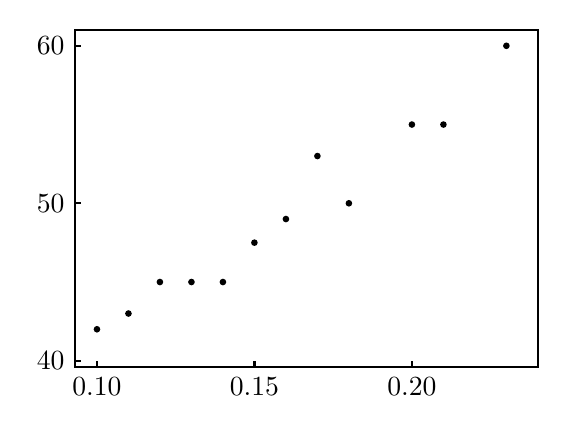
\begin{tikzpicture}[thick,x=40cm,y=0.2cm]
    \draw [thick] (0.093,39.6) -- (0.24,39.6) -- (0.24,61) -- (0.093,61) -- cycle;
    \draw (0.093,40)node[left]{40} -- ++(0.002,0) (0.093,50)node[left]{50} -- ++(0.002,0)
    (0.093,60)node[left]{60} -- ++(0.002,0);
    \draw (0.10,39.6)node[below]{0.10} -- ++(0,0.4)
    (0.15,39.6)  node[below] {0.15} -- ++(0,0.4)
    (0.20,39.6) node[below]{0.20} -- ++(0,0.4);
    \foreach \x/\y in {
      0.10/42, 0.11/43, 0.12/45, 0.13/45,
      0.14/45, 0.15/47.5, 0.16/49, 0.17/53,
      0.18/50, 0.20/55, 0.21/55, 0.23/60
    }
    \fill (\x,\y) circle(1.2pt);
  \end{tikzpicture}
        \caption{合金钢强度及碳含量的散点图}
        \label{fig:8.4.1}
    \end{figure}

    从散点图我们发现 $12$ 个点基本在一条直线附近, 这说明两个变量之间有一个线性相关关系, 若记 $y$ 轴方向上的误差为 $\varepsilon$, 这个相关关系可以表示为
    \begin{equation}
      y = \beta_0 + \beta_1 x + \varepsilon .
    \end{equation}
    这便是 $y$ 关于 $x$ 的一元线性回归的数据结构式. 这里总假定 $x$ 为一般变量, 是\textbf{非随机变量}\index{F!非随机变量}, 其值是可以精确测量或严格控制的, $\beta_0, \beta_1$ 为未知参数, $\beta_1$ 是直线的斜率, 它表示 $x$ 每增加一个单位 $E(y)$ 的增加量. $\varepsilon$ 是随机误差, 通常假定
    \begin{equation}\label{eq:8.4.3}
      E(\varepsilon) = 0, Var(\varepsilon) = \sigma^{2}.
    \end{equation}
    在对未知参数做区间估计或假设检验时, 还需要假定误差服从正态分布, 即
    \begin{equation}\label{eq:8.4.4}
      y \sim N(\beta_0 + \beta_1 x, \sigma^2)
    \end{equation}
    显然, 假定~\ref{eq:8.4.4} 比~\ref{eq:8.4.3} 要强.
    由 $\beta_0, \beta_1$ 均未知, 需要我们从收集到的数据 $(x_i, y_i), i=1,2, \cdots, n$ 出发进行估计. 在收集数据时, 我们一般要求观察独立地进行, 即假定 $y_{1}, y_{2},\cdots, y_{n}$ 相互独立. 综合上述诸项假定,我们可以给出最简单、常用的一元线性回归的统计模型:
    \begin{equation}\label{eq:8.4.5}
    \begin{cases}
      y_i = \beta _0 + \beta _1 + \varepsilon_{i} , \quad i =1, 2, \cdots, n; & \\
      \text{ 各 }\varepsilon_{i} \text{ 独立同分布, 其分布为 } N(0, \sigma^{2}) & \\
    \end{cases}
    \end{equation}
    由数据 $(x_{i}, y_{i}), i=1,2, \cdots, n$ ,可以获得 $\beta_0, \beta_1$ 的估计 $\hat{\beta}_0, \hat{\beta}_1$ 称
    \begin{equation}\label{eq:8.4.6}
    \hat{y} = \hat{\beta}_0 + \hat{\beta} _x
    \end{equation}
    为 $y$ 关于 $x$ 的\textbf{经验回归函数}\index{J!经验回归函数}, 简称为回归方程, 其图形称为回归直线. 给定 $x=x_0$ 后, 称 $ \hat{y}_{0} = \hat{\beta}_0 + \hat{\beta}_1 x_{0}$ 为\textbf{回归值}\index{H!回归值}(在不同场合也称其为拟合值、预测值).
\end{example}

\subsection{回归系数的最小二乘估计}\label{ssec:8.4.3}

一般采用最小二乘方法估计模型~\ref{eq:8.4.5} 中的 $\beta_0, \beta_1$. 令
\begin{equation*}
  Q(\beta_{0}, \beta_{1}) = \sum_{i=1}^{n} (y_{i} - \beta_{0} - \beta_{1} x_{i})^{2},
\end{equation*}
$\beta_0,\beta_1$ 应该满足
\begin{equation*}
  Q(\hat{\beta}_{0}, \hat{\beta}_{1}) =\min_{\beta_0, \beta_1} = Q(\beta_0, \beta_1),
\end{equation*}
称这样得到的 $\hat{\beta}_0, \hat{\beta}_1$ 称为 $\beta_0, \beta_1$ 为的最小二乘估计, 记为 LSE.

由于 $Q \ge 0$, 且对 $\beta_0, \beta_1$ 的导数存在, 因此最小二乘估计可以通过求偏导数并命其为 $0$ 而得到:
\begin{equation}\label{eq:8.4.7}
	\begin{cases}
	  \frac{\partial Q}{\partial \beta_{0}} = -2 \sum_{i=1}^{n}(y_{i} - \beta_{0} - \beta_{1} x_{i})=0 \\
		\frac{\partial Q}{\partial \beta_{1}} = -2 \sum_{i=1}^{n}(y_{i} - \beta_{0} - \beta_{1} x_{i}) x_{i}=0
	\end{cases}
\end{equation}
这组方程称为\textbf{正规方程组}\index{J!正规方程组}, 经过整理, 可得

\begin{equation}\label{eq:8.4.8}
	\begin{cases}
		n \hat{\beta}_{0} + n \bar{x} \hat{\beta}_{1} = n \bar{y} \\
		n \bar{x} \hat{\beta}_{0} + \sum x_{i}^{2} \hat{\beta}_{1} = \sum x_{i} y_{i}
	\end{cases}
\end{equation}
(今后凡是不作说明 $\sum$ 都表示 “$\sum_{i=1}^{n}$”). 记
\begin{equation*}
  \begin{split}
  \bar{x} & = \frac{1}{n}\sum x_{i}, \bar{y} = \frac{1}{n}\sum y_{i},\\
  l_{xy}  & =\sum(x_{i} - \bar{x}) (y_{i} - \bar{y}) =\sum x_{i} y_{i} - n \bar{x} \cdot \bar{y} =\sum x_{i} y_{i} - \frac{1}{n}\sum x_{i}\sum y_{i},\\
  l_{xx}  & =\sum(x_{i} - \bar{x})^{2} =\sum x_{i}^{2} - n \bar{x}^{2} =\sum x_{i}^{2} - \frac{1}{n}(\sigma x_{i})^{2}, \\
  l_{y y} & =\sum(y_{i} - \bar{y})^{2} =\sum y_{i}^{2} - n \bar{y}^{2} =\sum y_{i}^{2} - \frac{1}{n}(\sigma y_{i})^{2}.
  \end{split}
\end{equation*}
解~\ref{eq:8.4.8} 可得
\begin{equation}\label{eq:8.4.9}
  \begin{cases}
    \hat{\beta}_{1} = l_{xy}/l_{xx}, \\
    \hat{\beta}_{0} = \bar{y} - \hat{\beta}_{1} \bar{x}
  \end{cases}
\end{equation}
这就是参数的最小二乘估计, 其计算通常可列表进行, 见表~\ref{tab:8.4.2}.

\begin{example}\label{exam:8.4.2}
使用例~\ref{exam:8.4.1} 种合金钢强度和碳含量数据, 我们可求得回归方程, 见表~\ref{tab:8.4.1}.

\begin{table}[htbp]
  \centering
  \caption{例~\ref{exam:8.4.1} 的计算表\label{tab:8.4.2}}
  \begin{tabular}{ccc}
  \toprule
   $\sum x_i =1.90$          &     $n=12$                           & $\sum y_i = 590.5$       \\
   $\bar{x} = 0.1583$          &                                      & $\bar{y}  = 49.2083$       \\
   $\sum x_{i}^{2} = 0.3194$ & $ \sum x_iy_i=95.9250  $            & $\sum y_i^2 = 29392.75$  \\
   $ n \bar{x}^2 = 0.3008$     & $n\cdot\bar{x}\cdot\bar{y}=93.4958 $ & $n\bar{y}^2 = 29057.52$    \\
   $ l_{xx} = 0.0186$          & $l_{xy} = 2.4292$                    & $l_{yy}=335.23$            \\
   \midrule
   \multicolumn{3}{c}{ $\hat{\beta}_1 = l_{xy}/l_{xx} = 130.60$ }                                  \\
   \multicolumn{3}{c}{ $\hat{\beta}_0 = \bar{y} - \bar{x} \hat{\beta}_1=28.53$ }                   \\
   \bottomrule
  \end{tabular}%
\end{table}%

($l_{yy}$ 在后面将会用到)由此给出回归方程为
\begin{equation*}
  \hat{y} = 28.53 + 130.60 x
\end{equation*}
\end{example}

关于最小二乘估计的一些性质罗列在如下定理之中:
\begin{theorem}{}{8.4.1}
在模型~\ref{eq:8.4.5} 下, 有
\begin{enumerate}
  \item  $\hat{\beta}_{0} \sim N \left(\beta_{0}, \left(\frac{1}{n} + \frac{\bar{x}^{2}}{l_{xx}} \right)\sigma^2\right), \quad \hat{\beta}_{1} \sim N \left(\beta_{1}, \frac{\sigma^{2}}{l_{xx}} \right)$;\label{thm8.4.1.1}
  \item ${\operatorname{Cov}\left(\hat{\beta}_{0}, \hat{\beta}_{1}\right)=-\frac{\bar{x}}{l_{x x}}\sigma^2}$;\label{thm8.4.1.2}
  \item 对于给定的  $x_{0}, \hat{y}_{0}=\hat{\beta}_{0}+\hat{\beta}_{1} x_{0} \sim N\left(\beta_{0}+\beta_{1} x_{0},\left(\frac{1}{n}+\frac{\left(x_{0}-\bar{x}\right)^{2}}{l_{x x}}\right)\sigma^2\right) $.\label{thm8.4.1.3}
\end{enumerate}

\begin{proof}
利用 $\sum(x_i-\bar{x}) = 0$, 可把 $\hat{\beta}_{1}$ 和 $\hat{\beta}_{0}$ 改写为
  \begin{equation*}
    \begin{split}
      \hat{\beta}_{1} & = \frac{l_{zx}}{l_{xx}} =\sum \frac{x_{i} - \bar{x}}{l_{xx}} y_{i} \\
      \hat{\beta}_{0} & = \bar{y} - \hat{\beta}_{1} \bar{x} =\sum\left[\frac{1}{n} - \frac{(x_{i} - \bar{x}) \bar{x}}{l_{xx}}\right] y_{i}.
    \end{split}
  \end{equation*}
\end{proof}
它们是独立正态变量 $y_1,y_2, \cdots, y_n$ 的线性组合, 故都服从正态分布, 下面分别求其期望与方差
\begin{equation*}
\begin{split}
E(\hat{\beta}_{1}) & =\sum \frac{x_{i} - \bar{x}}{l_{xx}} E(y_{i}) =\sum \frac{x_{i} - \bar{x}}{l_{xx}}(\beta_{0} + \beta_{1} x_{i}) = \beta_{1}, \\
\Var(\hat{\beta}_{1}) & =\sum\left(\frac{x_{i} - \bar{x}}{l_{xx}} \right)^{2}  Var(y_{i}) =\sum \frac{(x_{i}-\bar{x})^{2}}{l_{xx}^{2}}\sigma^2 = \frac{\sigma^{2}}{l_{xx}} \\
E(\hat{\beta}_{0}) & = E(\hat{y}) - E(\hat{\beta}_{1}) \bar{x} = \beta_{0} + \beta_{1} \bar{x} - \beta_{1} \bar{x} = \beta_{0} \\
\Var(\hat{\beta}_{0}) & =\sum\left[\frac{1}{n} - \frac{(x_{i} - \bar{x}) \bar{x}}{l_{xx}}\right]^{2} \Var(y_{i}) = \left(\frac{1}{n} + \frac{\bar{x}^{2}}{l_{xx}}\right)\sigma^{2}.
\end{split}
\end{equation*}
这就证明了 \ref{thm8.4.1.1}. 进一步, 考虑到诸 $y_i$ 之间的独立性, 可得
\begin{equation*}
\begin{aligned}
\Cov(\hat{\beta}_{0}, \hat{\beta}_{1}) & = \Cov\left(\sum \left[\frac{1}{n}-\frac{(x_{i}-\bar{x})\bar{x}}{l_{x x}} \right] y_{i},\sum \frac{x_{i} -\bar{x}}{l_{xx}} y_{i}\right) \\
 & =\sum\left[\frac{1}{n}-\frac{(x_{i}-\bar{x}) \bar{x}}{l_{xx}}\right] \frac{x_{i}-\bar{x}}{l_{xx}}\sigma^{2} = - \frac{\bar{x}}{l_{xx}}\sigma^{2}.
\end{aligned}
\end{equation*}
这就证明了 \ref{thm8.4.1.2}. 为证明 \ref{thm8.4.1.3}, 注意到 $\hat{y}_0 = \hat{\beta}_0 + \hat{\beta}_1 x_0$ 也是 $y_1, y_2, \cdots, y_n$ 的线性组合, 它也服从正态分布, 只需求出其期望与方差即可.
\begin{equation*}
  \begin{split}
  E(\hat{y}_{0}) &= E(\hat{\beta}_{0}) + E(\hat{\beta}_{1}) x_{0} = \beta_{0} + \beta_{1} x_{0} = E(y_{0}) \\
  \Var(\hat{y}_{0}) &= \Var(\hat{\beta}_{0}) + \Var(\hat{\beta}_{1}) x_{0}^{2} + 2 Cov(\hat{\beta}_{0}, \hat{\beta}_{1}) \\
  & = \left[\left(\frac{1}{n}+\frac{\bar{x}^{2}}{l_{x x}}\right)+\frac{x_{0}^{2}}{l_{x x}}-2 \frac{x_{0} \bar{x}}{l_{x x}}\right]\sigma^{2}=\left[\frac{1}{n}+\frac{\left(x_{0}-\bar{x}\right)^{2}}{l_{x x}}\right]\sigma^{2}
  \end{split}
\end{equation*}
证明完成.
\end{theorem}

定理~\ref{thm:8.4.1} 说明:
\begin{itemize}
  \item  $\hat{\beta}_0, \hat{\beta}_1$ 分别是  $\beta_0, \beta_1$ 的无偏估计;
  \item  $\hat{y}_0$ 是 $E(y_0) =\beta_0 + \beta_1 x_1$ 的无偏估计;
  \item 除 $\bar{x}=0$ 外, $\hat{\beta}_0$ 与 $\hat{\beta}_1$ 是相关的.
  \item 要提高 $\hat{\beta}_0, \hat{\beta}_1$ 的估计精度(即降低它们的方差)就要求 $n$ 大, $l_{xx}$ 大(即要求 $x_1, x_2, \cdots, x_n$ 较分散).
\end{itemize}
% by ddswhu
\subsection{回归方程的显著性检验}\label{ssec:8.4.4}

从回归系数的 LSE 可以看出,对任意给出的 $n$ 对数据 $(x_i, y_i)$, 都可以求出 $\hat{\beta}_0, \hat{\beta}_1$, 从而给出回归方程 $\hat{y} = \hat{\beta }_0 + \hat{\beta }_1 x_{i}$, 但是这样给出的回归方程不一定有意义.

在使用回归方程作进一步的分析以前, 首先应对回归方程是否有意义进行判断. 什么叫回归方程有意义呢? 我们知道, 建立回归方程的目的是寻找 $y $ 的均值随 $x$ 变化的规律, 即找出回归方程 $E(y) = \beta _0 + \beta _1 x$. 如果 $\beta_1 = 0$, 那么不管 $x$ 如何变化, $E(y)$ 不随 $x$  的变化作线性变化, 那么这时求得的一元线性回归方程就没有意义, 称回归方程不显著. 如果 $\beta \neq 0$, 那么当 $x$ 变化时, $E(y)$ 随 $x$ 的变化作线性变化, 那么这时求得的回归方程就有意义, 称回归方程是显著的, 综上, 对回归方程是否有意义作判断就是要作如下的显著性检验:
\begin{equation*}
H_0:\beta_1=0 \quad \text{vs} \quad H_1:\beta_1 \neq 0
\end{equation*}
拒绝 $H_0$ 表示回归方程是显著的. 在一元线性回归中有三种等价的检验方法, 使用中只要任选其中之一即可.

\subsubsection{$F$ 检验}

采用方差分析的思想,我们从数据出发研究各 $y_i$ 不同的原因. 首先引入记号:记 $\hat{y}_i = \hat{\beta}_0 + \hat{\beta}_1 x$ 为\textbf{回归值}\index{H!回归值}, $y_i - \hat{y}_i$ 为\textbf{残差}\index{C!残差}.

数据总的波动用总偏差平方和
\begin{equation}\label{eq:8.4.10}
S_T=\sigma ( y_i - \bar{y}_i)^2 = l_{yy}
\end{equation}
表示. 引起各 $y_i$ 不同的原因主要有两个因素:其一是 $H_0$ 可能不真, $E(y)$ 随 $x$ 的变化而变化, 从而在每一个 $x$ 的观测值处的回归值不同, 其波动用回归平方和
\begin{equation}
S_R=\sigma{\left( \hat{y}_i-\bar{y}_i \right)}^2 \label{eq:8.4.11}
\end{equation}
表示;其二是其他一切因素, 包括随机误差、 $x$ 对 $E(y)$ 的非线性影响等,这样在得到回归值以后, $y$ 的观测值与回归值之间还有差距,这可用残差平方和
\begin{equation}
S_{e}=\sigma{\left( y_i-\hat{y}_i \right)}^2
\end{equation}
表示.
% modified
注意到 $\hat{\beta}_0, \hat{\beta}_1$ 满足正规方程组~\ref{eq:8.4.8}, 因此有
\begin{equation*}
\begin{array}{c}
\sum{\left( y_i-\hat{\beta }_0-\hat{\beta }_1x_i \right) =0\Rightarrow \sum{\left( y_i-\hat{y}_i \right)}}=0\\
\sum{\left( y_i-\hat{\beta }_0-\hat{\beta }_1x_i \right) x_i=0\Rightarrow \sum{\left( y_i-\hat{y}_i \right)}}x_i=0\\
\end{array}
\end{equation*}
利用 $\hat{y}_i=\hat{\beta }_0+\hat{\beta }_1x_i,x_i=\bar{y}+\hat{\beta }_1\left( x_i-\bar{x} \right) $ ,可得
\begin{equation*}
\begin{aligned}
\sum\left(y_{i}-\hat{y}_{i}\right)\left(\hat{y}_{i}-\bar{y}\right) &=\sum\left(y_{i}-\hat{y}_{i}\right)\left[\hat{\beta}_{1}\left(x_{i}-\bar{x}\right)\right] \\ &=\hat{\beta}_{1}\left[\sum\left(y_{i}-\hat{y}_{i}\right) x_{i}-\sum\left(y_{i}-\hat{y}_{i}\right) \bar{x}\right]=0
\end{aligned}
\end{equation*}
从而
\begin{equation*}
  S_{T} =\sum(y_{i}-\bar{y})^{2} =\sum(y_{i} - \hat{y}_{i} + \hat{y}_{i} - \bar{y})^{2} =\sum(y_{i} - \hat{y}_{i})^{2} +\sum(\hat{y}_{i}-\bar{y})^{2}
\end{equation*}
即
\begin{equation}
S_T = S_R + S_E, \label{eq:8.4.13}
\end{equation}
上式就是一元线性回归场合下的\textbf{平方和分解式}\index{P!平方和分解式}.

关于 $S_R$ 和 $S_e$ 所含有的成分可由如下定理说明.
\begin{theorem}{}{8.4.2}
    设  $y_i = \beta_0 + \beta_1 + \varepsilon_i$, 其中  $\varepsilon_1, \cdots, \varepsilon_n$ 相互独立, 且
    \begin{equation*}
    E(\varepsilon_i) = 0, \Var(y_i) = \sigma^2, i = 1, \cdots, n,
    \end{equation*}
    沿用上面的记号, 有
    \begin{align}
    E(S_R) =\sigma^2 + \beta_{1}^{2} l_{xx}\\
    E(S_e) = (n-2)\sigma^2,
    \end{align}
    这说明 $\hat{\sigma}^2 = S_{e}/(n-2)$ 是 $\sigma^2$ 的无偏估计.
\end{theorem}
\begin{proof}
    首先我们可以写出 $S_R$ 的简化公式:
    \begin{equation}
    S_{R}=\sum\left(\hat{y}_{i}-\bar{y}\right)^{2}=\sum\left[\bar{y}+\hat{\bar{\beta}}_{1}\left(x_{i}-\bar{x}\right)-\bar{y}\right]^{2}=\hat{\beta}_{1}^{2} l_{x x}
    \end{equation}\label{eq:8.4.16}
    从而
    \begin{equation*}
    \begin{aligned}
    E\left(S_{R}\right) &=E\left(\hat{\beta}_{1}^{2}\right) l_{x x}=\left[\Var\left(\hat{\beta}_{1}\right)+\left(E \hat{\beta}_{1}\right)^{2}\right] \cdot l_{x x} \\
    &=\left(\frac{\sigma^{2}}{l_{-x}}+\beta_{1}^{2}\right) l_{x x}=\sigma^{2}+\beta_{1}^{2} l_{x x}
    \end{aligned}
    \end{equation*}
    又
    \begin{equation*}
    \begin{aligned}
    S_{e}
    & =\sum\left(y_{i}-\hat{y}_{i}\right)^{2} \\
    & =\sum\left(\beta_{0}+\beta_{1} x_{i}+\varepsilon_{i}-\hat{\beta}_{0}-\hat{\beta}_{1} x_{i}\right)^{2}\\
    & =\sum\left[\left(\hat{\beta}_{0}-\beta_{0}\right)^{2}+x_{k}^{2}\left(\hat{\beta}_{1}-\beta_{1}\right)^{2}+\varepsilon_{i}^{2}+  2(\hat{\beta}_{0}-\beta_{0})\left(\hat{\beta}_{1}-\beta_{1}\right) x_{i}-\right.\\
    & \quad \left.2\left(\hat{\beta}_{0}-\beta_{0}\right) \varepsilon_{1}-2\left(\hat{\beta}_{1}-\beta_{1}\right) x_{i} \varepsilon_{i}\right]
    \end{aligned}
    \end{equation*}
    故
    \begin{equation*}
    \begin{array}{c}
    {E\left(S_{e}\right)=n \Var\left(\hat{\beta}_{0}\right)+\sum x_{i}^{2} \Var\left(\hat{\beta}_{1}\right)+n \Var(\varepsilon)+2 n \bar{x} \operatorname{Cov}\left(\hat{\beta}_{0}, \hat{\beta}_{1}\right)-} \\
    {2\sum E(\hat{\beta}_{0} \varepsilon_{i})-2\sum x_{i} E(\hat{\beta}_{1} \varepsilon_{i})}\end{array}
    \end{equation*}
    将 $\hat{\beta}_0, \hat{\beta}_i$ 写成 $y_1, y_2, \cdots, y_n$ 的线性组合, 利用 $y_i$ 与 $\varepsilon_i(i \neq j)$ 的独立性, 有
    \begin{equation*}
    \begin{split}
        E(\hat{\beta}_{0} \varepsilon_{i})& =E\left[\varepsilon_{i} \sum_{j}\left(\frac{1}{n}-\frac{\left(x_{j}-\bar{x}\right) \bar{x}}{l_{x x}}\right) y_{j}\right]=\left(\frac{1}{n}-\frac{\left(x_{i}-\bar{x}\right) \bar{x}}{l_{x x}}\right)\sigma^2\\
        E(\hat{\beta}_{1} \varepsilon_{i}) &=E\left[\varepsilon_{i} \sum_{j} \frac{x_{j}-\bar{x}}{l_{x x}} y_{j}\right]=\frac{x_{i}-\bar{x}}{l_{x x}}\sigma^2
    \end{split}
    \end{equation*}
    由此既有
    \begin{equation*}
   \sum E\left(\hat{\beta}_{0} \varepsilon_{i}\right)=\sigma^{2}, \quad\sum x_{i} E\left(\hat{\beta}_{1} \varepsilon_{i}\right)=\sigma^{2}
    \end{equation*}
    从而
    \begin{equation*}
    \begin{aligned} E\left(S_{e}\right) &=n\left[\frac{1}{n}+\frac{\bar{x}^{2}}{l_{x x}}\right]\sigma^2+\sum \frac{x_{i}^{2}}{l_{x x}}\sigma^{2} + n\sigma^2-\frac{2 n \bar{x}^{2}}{l_{x x}}\sigma^2-2\sigma^2-2\sigma^2 \\ &=(1+n-4)\sigma^2+\frac{1}{l_{x x}}\sum\left(x_{i}-\bar{x}\right)^{2}\sigma^2=(n-2)\sigma^2 \end{aligned}
    \end{equation*}
    这就完成了证明.
\end{proof}

进一步,有关 $S_R$ 和 $S_e$ 的分布,有如下定理.
\begin{theorem}{}{8.4.3}
设 $y_1\cdots,y_n$ 相互独立,且 $y_i\sim N(\beta_0+\beta_1x_i),i=1\cdots,n,$ 则在上述记号下,有
\begin{enumerate}
  \item  $S_e/\sigma^2 \sim \chi^2(n-2)$,
  \item  若 $H_0$ 成立, 则有 $S_R/\sigma^2 \sim \chi^{2}(1)$ ,
  \item  $S_R$ 与 $S_e$、$\bar{y}$ 独立(或 $\hat{\beta}_{1}$ 与 $S_e$、$\bar{y}$ 独立).
\end{enumerate}
\end{theorem}
\begin{proof}
取 $n \times n$ 的正交矩阵 $A$, 具有如下形式:
\begin{equation*}
A=\begin{pmatrix} & {a_{12}} & {\dots} & {a_{1 n}} \\ {\vdots} & {\vdots} & {} & {\vdots} \\ {a_{n-2,1}} & {a_{n-2,2}} & {\dots} & {a_{n-2, n}} \\ {\left(x_{1}-\bar{x}\right) / \sqrt{l_{x x}}} & {\left(x_{2}-\bar{x}\right) / \sqrt{l_{x x}}} & {\cdots} & {\left(x_{n}-\bar{x}\right) / \sqrt{l_{x x}}} \\ {1 / \sqrt{n}} & {1 / \sqrt{n}} & {\cdots} & {1 / \sqrt{n}}
\end{pmatrix}
\end{equation*}
由正交性, 可得如下一些约束条件
\begin{gather*}
\sum_{j} a_{i j}=0,\; \sum_{j} a_{i j} x_{j}=0,\;  \sum_{j} a_{i j}^{2}=1,\;  i = 1, 2, \cdots, n-2 \\
\sum_{k} a_{i k} a_{j k}=0, \quad 1 \leqslant i<j \leqslant n-2
\end{gather*}
这里共有 $n(n-2)$ 个未知参数, 约束条件有 $ 3(n-2)+\binom{n-2}{2} = (n - 2)(n + 3)/2$ 个, 只要 $n \ge 3$ , 未知参数个数就不少于约束条件数, 因此必定有解. 令
\begin{equation*}
Z=
\begin{pmatrix}
z_1\\
z_2\\
\vdots\\
x_n\\
\end{pmatrix}
=AY = A
\begin{pmatrix}
y_1\\
y_2\\
\vdots\\
y_n\\
\end{pmatrix}
=
\begin{pmatrix}
\sum_j{a}_{1j} y_{j}\\
\vdots\\
\displaystyle\sum_j{a}_{n-2, j} y_j\\
\displaystyle\sum_j{\frac{x_j-\bar{x}}{\sqrt{l_{xx}}}} y_j\\
\displaystyle\sum_j{\frac{1}{\sqrt{n}}} y_j\\
\end{pmatrix},
\end{equation*}
其中
\begin{equation*}
\begin{split}
z_{n-1} & = \frac{\sum(x_{t}-\bar{x}) y_{i}}{\sqrt{l_{x x}}} =
\frac{\sum(x_{i}-\bar{x})(y_{i}-\bar{y})}{\sqrt{l_{x x}}} =
\frac{l_{x y}}{\sqrt{l_{x x}}} =
\sqrt{l_{x x}} \hat{\beta}_{1}, \\
z_{n} & =\frac{1}{\sqrt{n}}\sum y_{i}=\sqrt{n} \bar{y}
\end{split}
\end{equation*}
则 ${Z}$ 仍然服从正态分布, 且其期望与协差阵分别为
\begin{equation*}
EZ =
  \begin{pmatrix}
    0      \\
    \vdots \\
    \beta_{1}\sqrt{l_{xx}} \\
    \sqrt{n}(\beta_{0} + \beta_{1} \bar{x}) \\
  \end{pmatrix},
  \quad
  \Var(Z) = A \Var(Y) A^{\mathrm{T}} =\sigma^2 I_{n},
\end{equation*}
这表明 $z_1, z_2, \cdots, z_n$ 相互独立, $z_1, z_2, \cdots, z_{n-2}$ 的共同分布为 $N(0,\sigma^2)$, $z_{n-1} \sim N(\beta_{1} \sqrt{l_{xx}},\sigma^2)$, $z_{n} \sim N(\sqrt{n} (\beta_0 + \beta_{1} \bar{x}),\sigma^2)$.

由于 $\sum z_{i}^{2} =\sum y_{i}^{2} = S_{T} + n \bar{y}^2 = S_{R} + S_{e} + n \bar{y}^2$, 而 $z_n = \sqrt{n} \bar{y}$, $z_{n-1} = \sqrt{l_{xx}}\hat{\beta}_{1} = \sqrt{S_{R}}$, 于是 $z_{1}^2 + z_{2}^2 + \cdots + z_{n-2}^2 = S_{e}$, 所以 $S_{e}, S_{R}, \bar{y}$ 三者相互独立,并有
\begin{equation*}
S_{e} /\sigma^2=\sum_{i=1}^{n-2}\left(z_{i} /\sigma^2\right) \sim \chi^{2}(n-2)
\end{equation*}
\begin{equation*}
\text{ 在 }\beta_{1}=0 \text { 时 }, S_{R} /\sigma^2=\left(z_{n-1} /\sum\right)^{2} \sim \chi^{2}(1)
\end{equation*}
证明完成.
\end{proof}

如同方差分析那样,我们可以考虑采用 $F$ 作为检验统计量:
\begin{equation*}
F=\frac{S_{R}}{S_{e} /(n-2)}
\end{equation*}
在 $\beta_1=0$ 时, $F\sim F(1,n-2)$ ,其中 $f_R=1,f_e=n-2$ .对于给定的显著性水平 $\alpha$ ,拒绝域为
\begin{equation*} F\ge F_{1-\alpha}(1,n-2).  \end{equation*}
整个检验也可列成一张方差分析表.
% by ddswhu
\begin{example}\label{exam:8.4.3}
在合金钢强度的例~\ref{exam:8.4.2} 中,我们已求出了回归方程, 这里我们考虑关于回归方程的显著性检验. 经计算有
\begin{equation*}
\begin{array}{ll}
{S_{T}=l_{y y}=335.23,} & {f_{T}=11} \\
{S_{R}=\hat{\beta}_{1}^{2} l_{x x}=130.60^{2} \times 0.0186=317.26,} & {f_{R}=1} \\ {S_{e}=S_{T}-S_{R}=335.23-317.26=17.97,} & {f_{e}=10}
\end{array}
\end{equation*}
把各平方和移人方差分析表, 继续进行计算, 具体见表~\ref{tab:8.4.3}.
% Table generated by Excel2LaTeX from sheet '1'
\begin{table}[htbp]
  \centering
  \caption{合金钢强度与碳含量回归方程的方差分析表}
  \begin{tabular}{ccccc}
      \toprule
      来源    &  平方和  & 自由度   & 均方和   & $ F$ 比 \\\midrule %
      回归    &  $S_R=317.26$  & $ f_R=1$   &  $MS_R=317.26$  &  $176.26$  \\
      残差    &  $S_e=17.97$  &  $f_e=10$  &  $MS_e=1.80$  &  \\\midrule
      总计    &  $S_T=335.23$  &  $f_T=11$  &       &  \\\bottomrule
  \end{tabular}%
  \label{tab:8.4.3}%
\end{table}%
若取 $\alpha=0.01$ ,则 $F_{0.99}(1,10)=10.0$. 由于 $176.55>10.0$, 因此, 在显著性水平 $0.01$ 下回归方程是显著的.
\end{example}

\subsubsection{$t$ 检验}


% by ddswhu
对 $H_0: \beta_1=0$ 的检验也可基于 $t$ 分布进行. 由于 $\hat{\beta}_{1} \sim N \left(\beta_{1}, \frac{\sigma^{2}}{l_{x x}}\right), \frac{S_{e}}{\sigma^{2}} \sim \chi^{2}(n-2)$ , 且与 $\hat{\beta}_1$ 相互独立, 因此在 $H_0$ 为真时, 有
\begin{equation}\label{eq:8.4.17}
t=\frac{\hat{\beta}_{1}}{\hat{\sigma} / \sqrt{l_{x x}}} \sim t(n-2)
\end{equation}
其中 $\hat{\sigma} =\sqrt{S_{e}/(n-2)}$, 由于 $\sigma_{\hat{\beta}_1}=\sigma/\sqrt{l_{xx}}$, 因此称 $\hat{\sigma}_{\hat{\beta}_1}=\hat{\sigma}/\sqrt{l_{xx}} $ 为 $\hat{\beta}_1$ 的标准误, 即 $\hat{\beta}_1$ 的标准差的估计. \eqref{eq:8.4.17} 式表示的 $t$ 统计量可用来检验假设 $H_0$ .对给定的显著性水平 $\alpha$ , 拒绝域为
\begin{equation*}
W= \left| |t| > t_{1-\alpha/2} (n-2) \right|
\end{equation*}

注意到 $t^2=F$ ,因此, $t$ 检验与 $F$ 检验是等同的.

以例~\ref{exam:8.4.2} 中数据为例, 可以计算得到
\begin{equation*}
t=\frac{130.6022}{\sqrt{1.7970} / \sqrt{0.0186}}=13.2872
\end{equation*}
若取 $\alpha=0.01$, 则 $t_{0.995}(10)=3.1698$, 由于 $13.2872>3.1698$, 因此, 在显著性水平 $0.01$ 下回归方程是显著的.

\subsubsection{相关系数检验}

当一元线性回归方程是反映两个随机变量 $x$ 与 $y$ 间的线性相关关系时,它的显著性检验还可通过对二维总体相关系数 $p$ 的检验进行.它的一对假设是
\begin{equation}\label{eq:8.4.18}
H_{0} : \rho=0 \quad \text { vs } \quad H_{1} : \rho \neq 0
\end{equation}
所用的检验统计量为样本相关系数
\begin{equation}\label{eq:8.4.19}
r=\frac{\sum\left(x_{i}-\bar{x}\right)\left(y_{i}-\bar{y}\right)}{\sqrt{\sum\left(x_{i}-\bar{x}\right)^{2}\sum\left(y_{i}-\bar{y}\right)^{2}}}=\frac{l_{x y}}{\sqrt{l_{x x} l_{y y}}}
\end{equation}
其中 $(x_i,y_i), i=1, \cdots, n$ 是容量为 $n$ 的二维样本.

利用施瓦茨不等式可以证明:样本相关系数也满足  $\left| r \right|\le 1$, 其中等号成立条件是存在两个实数 $a$ 与 $b$, 使得对 $i=1,\cdots, n$ 有 $y_i = a + b x_i$. 由此可见, $n$ 个点 $(x_{i}, y_{u}), i=1, \cdots, n$ 在散布图上的位置与样本相关系数 $r$ 有关, 譬如:
\begin{enumerate}
  \item  $r = \pm 1,n$ 个点完全在一条上升或下降的直线上;
  \item  $r > 0$, 当 $x$ 增加时, $y$ 有线性增加趋势,此时称正相关;
  \item  $r < 0$, 当 $x$ 增加时, $y$ 反而有线性减少趋势,此时称负相关;
  \item  $r = 0$, $n$ 个点可能毫无规律,也可能呈某种曲线趋势,此时称不相关.
\end{enumerate}

根据样本相关系数的上述性质, 检验~\eqref{eq:8.4.18} 中原假设 $H_0: \rho=0$ 的拒绝域为
\begin{equation*}
  W = \{|r| \geq c\},
\end{equation*}
其中临界值 $c$ 可由 $H_0:\rho =0$ 成立时样本相关系数的分布定出,该分布与自由度 $n-2$ 有关.

对给定的显著性水平 $\alpha$ ,由 $P(W)=P(|r|\ge c)=\alpha$ 知, 临界值 $c$ 应是 $H_0:\rho =0$ 成立下 $|r|$ 的分布的 $1-\alpha$ 分位数, 故记为 $c = r_{1-\alpha}(n-2)$. 我们还可以用 $F$ 分布来确定临界值 $c$, 下面加以叙述.

由样本相关系数的定义可以得到统计量 $r$ 与 $F$ 之间的关系
\begin{equation*}
r^{2} =\frac{l_{x y}^{2}}{l_{x x} l_{y y}}=\frac{S_{R}}{S_{T}}=\frac{S_{R}}{S_{R}+S_{e}}=\frac{S_{R} / S_{e}}{S_{R} / S_{e}+1}
\end{equation*}
而
\begin{equation*}
F=\frac{MS_R}{MS_e}=\frac{S_R}{S_e/\left( n-2 \right)}=\frac{\left( n-2 \right) S_R}{S_e}
\end{equation*}
两者综合,可得
\begin{equation*}
r^2=\frac{F}{F+(n-2)}
\end{equation*}
这表明, $|r|$ 是 $F$ 的严格单调增函数, 故可以从 $F$ 分布的 $1-\alpha$ 分位数 $F_{1-\alpha}(1,n-2)$ 得到 $|r|$ 的 $1-\alpha$ 分位数为
\begin{equation*}
c=r_{1-\alpha}(n-2)=\sqrt{\frac{F_{1-\alpha}(1, n-2)}{F_{1-\alpha}(1, n-2)+1}}
\end{equation*}
譬如,对 $\alpha =0.01,n=12$ ,查表知 $F_{0.99}(1,10)=10.04$ ,于是
\begin{equation*}
r_{0.99}(10)=\sqrt{\frac{10.04}{10.04+1}}=0.708
\end{equation*}
为实际使用方便, 人们已对 $r_{1-\alpha}(n-2)$ 编制了专门的表, 见附表 9.
以例~\ref{exam:8.4.2} 中数据为例,可以计算得到
\begin{equation*}
r=\frac{2.4292}{\sqrt{0.0186 \times 335.2292}}=0.9728
\end{equation*}

若取 $\alpha =0.01$, 查附表 9 知则 $r_{0.99}(10)=0.708$, 由于 $0.9728>0.708$, 因此, 在显著性水平 $0.01$ 下回归方程是显著的.


\subsection{估计与检测}\label{sec:8.4.5}

当回归方程经过检验是显著的后,可用来做估计和预测.这是两个不同的问题:
\begin{itemize}
    \item 当 $x=x_0$ 时,寻求均值 $E(y_0)=\beta_0+\beta_1 x_0$ 的点估计与区间估计(注意这里 $E(y_0)$ 是常量), 这是估计问题;
    \item 当 $x=x_0$ 时, $y_0$ 的观察值在什么范围内?由于 $y_0$ 是随机变量,为此只能求一个区间,使 $y_0$ 落在这一区间的概率为 $1-\alpha$ ,即要求 $\delta$ ,使 $P(|y_0-\hat{y}_0|<\delta)=1-\alpha$ ,称区间 $\left[\hat{y}_{0}-\delta, \hat{y}_{0}+\delta\right]$ 为 $y_0$ 的概率为 $1-\alpha$ 的预测区间,这是预测问题.
\end{itemize}

\subsubsection{$E(y_0)$ 的估计}


在 $x=x_0$ 时,其对应的因变量 $y_0$ 是一个随机变量,有一个分布,我们经常需要对该分布的均值给出估计.我们知道,该分布的均值 $E(y_0)=\beta_0+\beta_1x_0$ ,因此,一个直观的估计应为
\begin{equation*}
\hat{E}(y_{0})=\hat{\beta}_0+\hat{\beta}_1 x_0
\end{equation*}
简单起见,我们习惯上将上述估计记为 $\hat{y}_0$ (注意这里 $\hat{y}_0$ 表示的是 $E(y_0)$ 的估计,而不表示 $y_0$ 的估计,因为 $y_0$ 是随机变量,它是没有估计的).由于 $\hat{\beta}_0,\hat{\beta}_1$ 分别是 $\beta_0,\beta_1$ 的无偏估计,因此 $\hat{y}_0$ 也是 $E(y_0)$ 的无偏估计.

为得到 $E(y_0)$ 的区间估计,我们需要知道 $\hat{y}_0$ 的分布.由定理~\ref{thm:8.4.1} 可得
\begin{equation*}
\hat{y}_{0}=\hat{\beta}_{0}+\hat{\beta}_{1} x_{0} \sim N\left(\beta_{0}+\beta_{1} x_{0},\left[\frac{1}{n}+\frac{\left(x_{0}-\bar{x}\right)^{2}}{l_{x x}}\right]\sigma^2\right)
\end{equation*}
又由定理~\ref{thm:8.4.3} 知, $S_{e} /\sigma^2 \sim \chi^{2}(n-2)$,且与 $\hat{y}_{0}=\bar{y}+\hat{\beta}_{1}\left(x_{0}-\bar{x}\right)$ 相互独立,记
\begin{equation*}
\hat{\sigma}^2=\frac{S_e}{n-2}
\end{equation*}
则
\begin{equation*}
\frac{\left(\hat{y}_{0}-E y_{0}\right) / \sqrt{\frac{1}{n}+\frac{\left(x_{0}-\bar{x}\right)^{2}}{l_{x x}}}\sigma }{\sqrt{\frac{S_{e}}{\sigma^{2}} /(n-2)}}=\frac{\hat{y}_{0}-E y_{0}}{\hat{\sigma} \sqrt{\frac{1}{n}+\frac{\left(x_{0}-\bar{x}\right)^{2}}{l_{x x}}}}-t(n-2)
\end{equation*}
于是 $E(y_0)$ 的 $1 - \alpha$ 的置信区间是
\begin{equation}\label{eq:8.4.20}
\left[ \hat{y}_0-\delta _0,\hat{y}_0+\delta _0 \right]
\end{equation}
其中
\begin{equation}
\delta_{0}=t_{1-\alpha / 2}(n-2) \hat{\sigma} \sqrt{\frac{1}{n}+\frac{\left(x_{0}-\bar{x}\right)^{2}}{l_{x x}}}\label{eq:8.4.21}
\end{equation}

\subsubsection{$y_0$ 的预测区间}

\eqref{eq:8.4.20} 给出了 $x=x_0$ 时对应的因变量的均值 $E(y_0)$ 的区间估计,实用中往往更关心 $x=x_0$ 时对应的因变量 $y_0$ 的取值范围.我们举一个不是非常贴切的例子说明这两者之间的差别:设想你要去买一台某厂生产的某种型号的彩电,则你很关心彩电的寿命—它能正常使用多长时间,彩电的寿命是一个随机变量,该厂生产的该型号的彩电寿命有一个分布,其均值就是它的平均寿命,当然,这是一个重要的质量指标,我们可以对它给出估计,譬如,平均寿命的 $0.95$ 置信区间为 $(12,18)$ (单位:千小时).然而,作为消费者,我们更关心的可能是我所购买的这台彩电的寿命在一个什么范围内,我所购买的这台彩电的寿命是一个随机变量,我们能否对该随机变量的取值给出一个预测区间呢?这就是我们这里要讨论的预测问题.

事实上, $y_0=E(y_0)+\varepsilon$ ,由于通常假定 $\varepsilon\sim N(0,\sigma^2)$ ,因此, $y_0$ 的最可能取值仍然为 $y_0$ ,于是,我们可以使用以列为中心的一个区间
\begin{equation}\label{eq:8.4.22}
\left( \hat{y}_0-\delta ,\hat{y}_0+\delta \right)
\end{equation}
作为 $y_0$ 的取值范围,为确定 $\delta$ 的值, 我们需要如下的结果:由于 $y_0$ 与 $\hat{y}_0$ 独立,故
\begin{equation*}
y_{0}-\hat{y}_{0} \sim N\left(0,\left[1+\frac{1}{n}+\frac{\left(x_{0}-\bar{x}\right)^{2}}{l_{x x}}\right]\sigma^2\right).
\end{equation*}
因此有
\begin{equation*}
\frac{y_{0}-\hat{y}_{0}}{\hat{\sigma} \sqrt{1+\frac{1}{n}+\frac{\left(x_{0}-\bar{x}\right)^{2}}{l_{x x}}}} \sim t(n-2)
\end{equation*}
从而~\eqref{eq:8.4.22} 表示的预测区间中 $\delta$ 的表达式为:
\begin{equation}
\delta=\delta\left(x_{0}\right)=t_{1-a / 2}(n-2) \hat{\sigma} \sqrt{1+\frac{1}{n}+\frac{\left(x_{0}-\bar{x}\right)^{2}}{l_{x x}}}.\label{eq:8.4.23}
\end{equation}
上述预测区间与 $E(y_0)$ 的置信区间~\eqref{eq:8.4.21} 的差别就在于根号里多个 $1$ ,计算时要注意到这个差别,这个差别导致预测区间要比置信区间宽一些.

由~\eqref{eq:8.4.23} 式可以看出预测区间的长度 $2\delta$ 与样本量 $n$, $x$ 的偏差平方和 $l_{xx}$, $x_0$ 到 $\bar{x}$ 的距离 $|x_0 - \bar{x}|$ 有关. $x_0$ 愈远离 $\bar{x}$ 预测精度就愈差.当 $x_0 \notin [x_{(1)},x_{(n)}]$ 时, 预测精度可能变得很差, 在这种情况下的预测称作外推,需要特别小心.另外,若 $x_{1}, x_{2}, \cdots, x_{n}$ 较为集中时, 那么 $l_{xx}$ 就较小,也会导致预测精度的降低.因此,在收集数据时要使 $x_{1}, x_{2}, \cdots, x_{n}$ ,尽量分散,这对提高精度有利.图~\ref{fig:8.4.2.a}
给出在不同的 $x$ 值上预测区间的示意图:在 $x=\bar{x}$ 处预测区间最短,远离乏的预测区间愈来愈长,呈喇叭状.
\begin{figure}[htb!]
    \begin{minipage}[b]{0.5\textwidth}
        \centering
        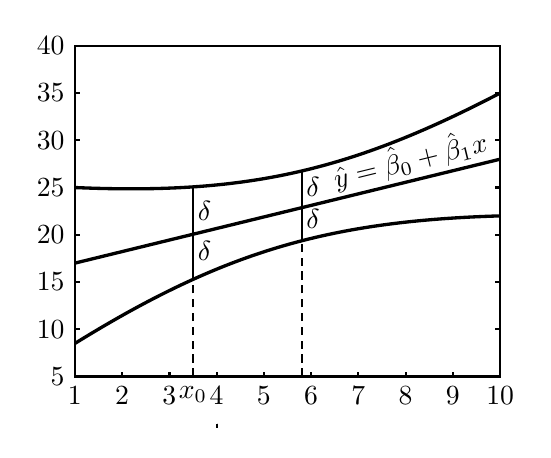
\begin{tikzpicture}[thick,x=0.6cm,y=0.12cm]
    \draw (1,5) -- (10,5) --  (10,40) -- (1,40) -- cycle;
    \foreach \x in {1,...,10}
      \draw (\x,5) node[below] {\x} -- ++ (0,0.5)
      (4,0) -- ++ (0,-0.5);
    \foreach \y in {5,10,...,40}
       \draw (1,\y)node[left]{\y} -- ++ (0.1,0) (10,\y) -- ++ (-0.1,0);
    \draw [very thick] (1,8.5) [bend left = 15] to (10,22);
    \draw [very thick] (1,17) -- node[sloped,pos=0.8,above=-2pt]{$\hat y=\hat\beta_0+\hat\beta_1x$} (10,28);
    \draw [very thick] (1,25) [bend right = 15] to (10,35);
    \draw [densely dashed] (3.5,5)node[below] {$x_0$} -- ++ (0,10.4)coordinate(a) (5.8,5) -- ++ (0,14.5)coordinate(b);
    \draw (a) -- node[right=-2pt,pos=0.3]{$\delta$}
    node [right=-2pt,pos=0.75]{$\delta$} ++ (0,9.5) ;
    \draw (b) -- node[right=-2pt,pos=0.3]{$\delta$}
    node [right=-2pt,pos=0.75]{$\delta$} ++ (0,7.4);
  \end{tikzpicture}
        \subcaption{精确预测区间\label{fig:8.4.2.a}}
    \end{minipage}
    \begin{minipage}[b]{0.45\textwidth}
        \centering
        \begin{tikzpicture}[>=Stealth,thick]
    \draw [Stealth-Stealth] (0,4) -- (0,0) node[below left] {$O$} -- (4,0);
    \draw [very thick] plot [domain = 0.5:3.5] (\x, 0.5*\x+2.6);
    \draw [very thick] plot [domain = 0.5:3.7] (\x, 0.5*\x+1.8);
    \draw [very thick] plot [domain = 0.7:3.9] (\x, 0.5*\x+1);
    \draw [densely dashed] (1.2,0) -- ++ (0,1.6) coordinate(a)
        (2.8,0) -- ++ (0,2.4) coordinate(b);
    \draw (a) -- node [right] {$\delta$}  ++ (0,0.8)
              -- node [right] {$\delta$}  ++ (0,0.8)
          (b) -- node [right] {$\delta$}  ++ (0,0.8)
              -- node [right] {$\delta$}  ++ (0,0.8);
    \node at (4.1,3.2) {$\hat y=\hat\beta_0+\hat\beta_1x$};
  \end{tikzpicture}
        \subcaption{近似预测区间\label{fig:8.4.2.b}}
    \end{minipage}
    \caption{预测区间示意图}\label{fig:8.4.2}
\end{figure}

当 $n$ 较大时(如 $n>30$ ), $t$ 分布可以用正态分布近似,进一步,若 $x_0$ 与 $\bar{x}$ 相差不大时, $\delta$ 可以近似取为:
\begin{equation}\label{eq:8.4.24}
\delta \approx \hat{\sigma} u_{1-\alpha/2}
\end{equation}
其中 $u_{1-\alpha/2}$ 是标准正态分布的 $1-\alpha/2$ 分位数, 见图~\ref{fig:8.4.2.b}.

\begin{example}
    在例~\ref{exam:8.4.2} 中,如果 $x_0=0.16$ ,则得预测值为
    \begin{equation*}\label{eq:8.4.25}
    y_0=28.5364+130.6022 \times 0.16=49.4328.
    \end{equation*}
    若取 $\alpha=0.05$ ,则 $t_{0.975}(10)=2.2281$ ,又 $\hat{\sigma}=\sqrt{17.9703/(12-2)}=1.3405$ , 应用~\eqref{eq:8.4.21},
    \begin{equation*}
    \delta_{0}=1.3405 \times 2.2281 \times \sqrt{\frac{1}{12}+\frac{(0.16-0.19)^{2}}{0.0186}}=1.08.
    \end{equation*}
    故 $x_0=0.16$ 对应因变量 $y_0$ 的均值 $E(y_0)$ 的 $0.95$ 置信区间为
    \begin{equation*}
    49.43\pm 1.08=\left( 48.35,50.51 \right).
    \end{equation*}
    应用~\eqref{eq:8.4.23},
    \begin{equation*}
    \delta=1.3405 \times 2.2281 \times \sqrt{1+\frac{1}{12}+\frac{(0.16-0.19)^{2}}{0.0186}}=3.18,
    \end{equation*}
    从而 $y_0$ 的概率为 $0.95$ 的预测区间为
    \begin{equation*}
    49.43\pm 3.18=(46.25,52.61).
    \end{equation*}
    我们可以清楚地看到, $E(y_0)$ 的 $0.95$ 置信区间比 $y_0$ 的概率为 $0.95$ 的预测区间窄很多,这是因为随机变量的均值相对于随机变量本身而言要更容易估计出来.

    如果求近似预测区间,则可按~\eqref{eq:8.4.24} 计算,由于 $u_{0.975}=1.96$ ,故有 $\delta\approx 1.96\times 1.34=2.63$ ,则所求区间为
    \begin{equation*}
    (49.43-2.63,49.43+2.63)=(46.80,52.06).
    \end{equation*}
    此处近似预测区间与精确预测区间相差较大,主要是因为 $n$ 较小的原因.
\end{example}

下而我们以一个完整的例子把本节内容重新梳理一遍.
\begin{example}\label{exam:8.4.5}
    在动物学研究中,有时需要找出某种动物的体积与重量的关系. 因为动物的重量相对而言容易测量,而测量体积比较困难, 因此, 人们希望用动物的重量预测其体积.下面是 $18$ 只某种动物的体积与重量数据,在这里,动物重量被看作自变量,用 $x$ 表示,单位为 $\si{\kilogram}$ ,动物体积则作为因变量,用 $y$ 表示,单位为 $\mathrm{dm}^3$, 18 组数据列于表~\ref{tab:8.4.4} 中.
    % Table generated by Excel2LaTeX from sheet '1'
    \begin{table}[htbp]
        \centering
        \caption{ $18$ 只某种动物的重量 $x$ 与体积 $y$ 数据}
        \begin{tabularx}{0.8\linewidth}{ZZ|ZZ|ZZ}
            \toprule
            $x$     & $y$     & $x$     & $y$     & $x$     & $y$ \\ \midrule
            10.4  & 10.2  & 15.1  & 14.8  & 16.5  & 15.9  \\
            10.5  & 10.4  & 15.1  & 15.1  & 16.7  & 16.6  \\
            11.9  & 11.6  & 15.1  & 14.5  & 17.1  & 16.7  \\
            12.1  & 11.9  & 15.7  & 15.7  & 17.1  & 16.7  \\
            13.8  & 13.5  & 15.8  & 15.2  & 17.8  & 17.6  \\
            15.0  & 14.5  & 16.0  & 15.8  & 18.4  & 18.3  \\ \bottomrule
        \end{tabularx}%
        \label{tab:8.4.4}%
    \end{table}%

    为能用动物重量估计动物体积,必须建立动物体积 $y$ 关于动物重量 $x$ 的回归方程. 首先,我们用这 $18$ 组数据画出散点图,见图~\ref{fig:8.4.3}.
    \begin{figure}[!htb]
        \centering
        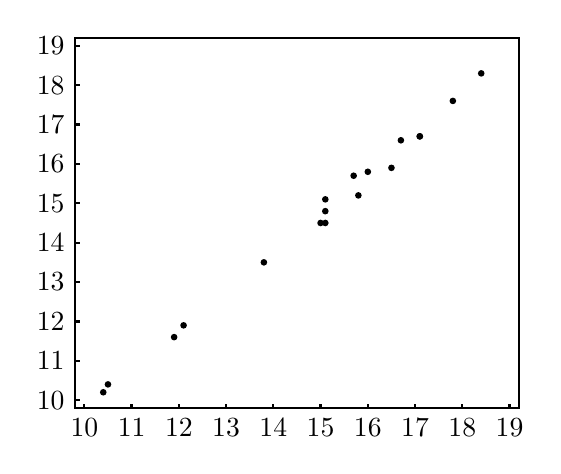
\begin{tikzpicture}[x=0.6cm,y=0.5cm,thick]
    \draw (9.8,9.8) -- (19.2,9.8) -- (19.2,19.2)--
       (9.8,19.2) -- cycle;
    \foreach \x in {10,11,...,19}
      \draw (\x,9.8) node[below] {\x} -- ++ (0,0.1)
            (9.8,\x) node[left] {\x} -- ++ (0.1,0);
    \foreach \x/\y in {
      10.4/10.2, 10.5/10.4, 11.9/11.6, 12.1/11.9,
      13.8/13.5, 15.0/14.5, 15.1/14.8, 15.1/15.1,
      15.1/14.5, 15.7/15.7, 15.8/15.2, 16.0/15.8,
      16.5/15.9, 16.7/16.6, 17.1/16.7, 17.1/16.7,
      17.8/17.6, 18.4/18.3
    }
    \fill (\x,\y) circle(1.2pt);
  \end{tikzpicture}
        \caption{动物体积与动物重量的散点图}
        \label{fig:8.4.3}
    \end{figure}

    从散点图我们发现 $18$ 个点基本在一条直线附近,这说明两个变量之间有一个线性相关关系,下面求该线性回归方程,计算过程见表~\ref{tab:8.4.5}.
    % Table generated by Excel2LaTeX from sheet '1'
    \begin{table}[htbp]
      \renewcommand*{\arraystretch}{1.5}
        \centering
        \caption{例~\ref{exam:8.4.5} 的计算表}
        \begin{tabular}{ccc}
          \toprule
         $\sum x_i=270.1$   &    $n=18$     &  $\sum y_i=265.0$  \\
         $\bar{x}=15.0056$   &       &  $\bar{y}=14.7222$  \\
         $\sum x_{i}^{2}=4149.39$   &    $\sum x_iy_i=4071.71$     &  $\sum y_{i}^{2}=3996.14$  \\
         $n\bar{x}^2=4053.0006$   &    $n \cdot\bar{x} \cdot \bar{y}=39976.422$     &  $n\bar{y}^2=3901.3889$  \\
         $l_{xy}=96.3894$   &    $l_{xy}=95.238$     &  $l_{yy}=94.7511$  \\
         \midrule
            \multicolumn{3}{c}{ $\hat{\beta}_1=l_{xy}/l_{xx}=0.9881$ } \\
            \multicolumn{3}{c}{ $\hat{\beta}_0=\bar{y}-x\hat{\beta}_1=-0.1048$ } \\
        \bottomrule
        \end{tabular}%
        \label{tab:8.4.5}%
    \end{table}%


    由此给出回归方程为
    \begin{equation}
    \hat{y}= - 0.1048 + 0.9881x. \label{eq:8.4.25}
    \end{equation}
    接下来我们考虑关于回归方程的显著性检验. 经计算有
    \begin{equation*}
    \begin{array}{ll}{S_{T}=l_{y y}=94.751,} & {f_{T}=17} \\ {S_{R}=\hat{\beta}_{1}^{2} l_{x x}=0.9881^{2} \times 96.3894=94.1090,} & {f_{R}=1} \\ {S_{e}=S_{T}-S_{R}=0.6421,} & {f_{e}=16}\end{array}
    \end{equation*}
    把诸平方和移入方差分析表上,继续计算,具体见表~\ref{tab:8.4.6}.
    \begin{table}[htbp]
        \centering
        \caption{合金钢强度与碳含量回归方程的方差分析表}
        \begin{tabular}{ccccc}
            \toprule
            来源    &  平方和  & 自由度   & 均方和   & $ F$ 比 \\\midrule %
            回归    &  $S_R=94.4090$  & $ f_R=1$   &  $MS_R=94.1090$  &  $2346.9$  \\
            残差    &  $S_e=0.6421$  &  $f_e=16$  &  $MS_e=0.0401$  &  \\\midrule
            总计    &  $S_T=94.7511$  &  $f_T=17$  &       &  \\\bottomrule
        \end{tabular}%
        \label{tab:8.4.6}%
    \end{table}%

  \noindent 若取 $\alpha=0.01$ ,则 $F_{0.99}(1,10)=8.53$ ,由于 $2346.9>8.53$ ,因此,在显著性水平 $0.01$ 下回归方程是显著的.

    如果测得某动物的重量为 $x_0=17.6\si{\kilogram}$ ,则由~\eqref{eq:8.4.25}, 该动物体积的估计值为
    \begin{equation*}
    \hat{y}_{0}=-0.1048+0.9881 \times 17.6=17.2858
    \end{equation*}

    若取 $\alpha=0.05$ ,则 $t_{0.975}(16)=2.1199$ ,又 $\hat{\sigma}=\sqrt{0.0401}=0.2002$ ,应用~\eqref{eq:8.4.21}
    \begin{equation*}
    \delta=0.2002 \times 2.1199 \times \sqrt{1+\frac{1}{18}+\frac{(17.6-15.0056)^{2}}{96.3894}}=0.4776
    \end{equation*}
    从而该动物体积的概率为 $0.95$ 的预测区间为
    \begin{equation*}
      (17.2858 - 0.4776, 17.2858 + 0.4776)=(16.8082, 17.7634).
    \end{equation*}

    用~\eqref{eq:8.4.24}可以求近似预测区间, 由于 $u_{0.975}=1.96$ ,故有 $\delta \approx 1.96\times 0.2002=0.3924$, 则所求区间为
    \begin{equation*}
    (17.2858 - 0.392 4, 17.2858 + 0.3924)=(16.8934,17.6782).
    \end{equation*}
    此处近似预测区间与精确预测区间差距已不大了,当 $n$ 更大一些,两者差距会更小一些.
\end{example}

\begin{xiti}
    \item 假设回归直线过原点,即一元线性回妇模型为
    \begin{equation*}
    y_i=\beta x_i+\varepsilon_i,\quad i=1,\cdots ,n,
    \end{equation*}
 $E(\varepsilon_i)=0, \Var(\varepsilon_i)=\sigma^2$ ,诸观测值相互独立.
    \begin{enumerate}
        \item 写出 $\beta,\sigma^2$ 的最小二乘估计;
        \item 对给定的 $x_0$ ,其对应的因变量均值的估计为 $\hat{y}_0$ ,求 $\Var(\hat{y}_0)$ .
    \end{enumerate}
    \item 设回归模型为
    \begin{equation*}
      \begin{cases}
        y_i=\beta _0+\beta _1x_i+\varepsilon _i,i=1,2,\cdots ,n,\\
    \text{各 $\varepsilon$ 独立同分布}, \text{其分布为} N(0,\sigma^2)
      \end{cases}
    \end{equation*}
    试求 $\beta_0,\beta_1,\sigma^2$ 的最大似然估计,它们与其最小二乘估计一致吗?
    \item 在回归分析计算中,常对数据进行变换:
    \begin{equation*}
    \tilde{y}_{\mathrm{i}}=\frac{y_{i}-c_{1}}{d_{1}}, \tilde{x}_{i}=\frac{x_{i}-c_{2}}{d_{2}}, i=1, \cdots, n
    \end{equation*}
    其中 $c_1,c_2,d_1(>0),d_2(>0)$ 是适当选取的常数.
    \begin{enumerate}
        \item 试建立由原始数据和变换后数据得到的最小二乘估计、总平方和、回归平方和以及残差平方和之间的关系;
        \item 证明:由原始数据和变换后数据得到的 $F$ 检验统计量的值保持不变.
    \end{enumerate}
    \item 对给定的 $n$ 组数据 $(x_{i}, y_{i}),i=1,\cdots,n$, 若我们关心的是 $y$ 如何依赖 $x$ 的取值而变动,则可以建立如下回归方程\begin{equation*}
    \hat{y}=a+bx.
    \end{equation*}
    反之,若我们关心的是 $x$ 如何依赖 $y$ 的取值而变动,则可以建立另一个回归方程
    \begin{equation*}
    \hat{x}=c+dy.
    \end{equation*}
    试问这两条直线在直角坐标系中是否重合?为什么?若不重合,它们有无交点?若有,试给出交点的坐标.
    \item 为考察某种维尼纶纤维的耐水性能,安排了一组试验,测得其甲醇浓度 $x$ 及相应的
    “缩醇化度” $y$ 数据如下:
    % Table generated by Excel2LaTeX from sheet '1'
    \begin{equation*}
    \begin{array}{c|ccccccc}
    x     & 18    & 20    & 22    & 24    & 26    & 28    & 30 \\\hline
    y     & 26.86  & 28.35  & 28.75  & 28.87  & 29.75  & 30.00  & 30.36  \\
    \end{array}%
    \end{equation*}
    \begin{enumerate}
        \item 作散点图;
        \item 求样本相关系数;
        \item 建立一元线性回归方程;
        \item 对建立的回归方程作显著性检验 $(\alpha=0.05)$ .
    \end{enumerate}
    \item 测得一组弹簧形变 $x$ (单位: $\si{cm}$ )和相应的外力 $y$ (单位: $\si{N}$ )数据如下:% Table generated by Excel2LaTeX from sheet '1'
    \begin{equation*}
    \begin{array}{c|cccccccccc}
    x     & 1.0   & 1.2   & 1.4   & 1.6   & 1.8   & 2.0   & 2.2   & 2.4   & 2.8   & 3.0  \\\hline
    y     & 3.08  & 3.76  & 4.31  & 5.02  & 5.51  & 6.25  & 6.74  & 7.40  & 8.54  & 9.24  \\
    \end{array}%
    \end{equation*}
    由胡克定律知 $y=kx$ ,试估计 $k$ ,并在 $x=2.6 \si{cm}$ 试给出相应的外力 $y$ 的 $0.95$ 预测区间.
    \item 设由 $(x_i,y_i),i=1,\cdots,n$ 可建立一元线性回归方程,,是由回归方程得到的拟合值,证明:样本相关系数 $r$ 满足如下关系
    \begin{equation*}
    r^{2}=\frac{\sum_{i=1}^{n}\left(y_{i}-\bar{y}\right)^{2}}{\sum_{i=1}^{n}\left(y_{i}-\bar{y}\right)^{2}}
    \end{equation*}
    上式也称为回归方程的决定系数.
    \item 现收集了 $16$ 组合金钢中的碳含量 $x$ 及强度 $y$ 的数据,求得
    \begin{equation*}
    \bar{x}=0.125, \quad y=45.7886,\quad l_{xx}=0.3024,\quad l_{xy}=25.5218,\quad l_{yy}=2432.4566.
    \end{equation*}
    \begin{enumerate}
        \item  建立 $y$ 关于 $x$ 的一元线性回归方程 $\hat{y}=\hat{\beta}_0+\hat{\beta}_1x$ ;
        \item 写出 $\hat{\beta}_0$ 和 $\hat{\beta}_1$ 的分布;
        \item 求 $\hat{\beta}_0$ 和 $\hat{\beta}_1$ 的相关系数;
        \item 列出对回归方程做显著性检验的方差分析表 $(\alpha=0.05)$ ;
        \item 给出 $\beta_1$ 的 $0.95$ 置信区间;
        \item 在 $x=0.15$ 时求对应的 $y$ 的 $0.95$ 预测区间.
    \end{enumerate}
    \item 设回归模型为 $\left\{\begin{aligned}
          & y_i=\beta_{0}+\beta_{1} x_{1}+\varepsilon_{i}, \\
          & \varepsilon_{i} \sim N\left(0,\sigma^2\right),
          \end{aligned}\right.$ 现收集了 $15$ 组数据,经计算有
    \begin{equation*}
    \bar{x}=0.85 \quad \bar{y}=25.60, \quad l_{x x}=19.56, \quad l_{x y}=32.54, \quad l_{x y}=46.74
    \end{equation*}
    后经核对,发现有一组数据记录错误,正确数据为 $(1.2,32.6)$ ,记录为 $(1.5,32.3)$ .
    \begin{enumerate}
        \item 求 $\beta_0,\beta_1$ 的 $\mathrm{LSE}$ ;
        \item 对回归方程做显著性检验 $(\alpha=0.05)$ ;
        \item 若 $x_0=1.1$ ,给出对应响应变量的 $0.95$ 预测区间.
    \end{enumerate}
    \item 在生产中积累了 $32$ 组某种铸件在不同腐蚀时间 $x$ 下腐蚀深度 $y$ 的数据,求得回归方程为
    \begin{equation*}
    \hat{y}=-0.4441+0.002263x
    \end{equation*}
    ,且误差方差的无偏估计为 $\hat{\sigma}^2=0.001452$, 总偏差平方和为 $0.1246$ .
    \begin{enumerate}
        \item 对回归方程做显著性检验 $(\alpha=0.05)$ ,列出方差分析表;
        \item 求样本相关系数;
        \item 若腐蚀时间 $x=870$ ,试给出 $y$ 的 $0.95$ 近似预测区间.
    \end{enumerate}
    \item 我们知道营业税税收总额 $y$ 与社会商品零售总额 $x$ 有关,为能从社会商品零售总额去预测税收总额,需要了解两者之间的关系.现收集了如下九组数据:(单位:亿元)
    \begin{equation*}
    \begin{array}{ccc}
    \toprule
    \text{序号}    & \text{社会商品零售额} & \text{营业税收总额} \\\midrule
    1     & 142.08  & 3.93  \\
    2     & 177.30  & 5.96  \\
    3     & 204.68  & 7.85  \\
    4     & 242.68  & 9.82  \\
    5     & 316.24  & 12.50  \\
    6     & 341.99  & 15.55  \\
    7     & 332.69  & 15.79  \\
    8     & 389.29  & 16.39  \\
    9     & 453.40  & 18.45  \\\bottomrule
    \end{array}%
    \end{equation*}
    \begin{enumerate}
        \item 画散点图;
        \item 建立一元线性回归方程,并做显著性检验(取 $\alpha=0.05$ ),列出方差分析表;
        \item 若已知某年社会商品零售额为 $300$ 亿元,试给出营业税税收总额的概率为 $0.95$ 的预测区间;
        \item 若已知回归直线过原点,试求回归方程,并在显著性水平 $0.05$ 下做显著性检验.
    \end{enumerate}
\end{xiti}

\section{一元非线性回归}\label{sec:8.5}

有时,回归函数并非是自变量的线性函数,但通过变换可以将之化为线性函数,从而利用一元线性回归对其分析,这样的问题是非线性回归问题.下面以一个例子说明上述非线性回归的分析步骤.
\begin{example}
    炼钢厂出钢水时用的钢包,在使用过程中由于钢水及炉渣对耐火材料的侵蚀,其容积不断增大.现在钢包的容积用盛满钢水时的质量 $y$ kg 表示,相应的试验次数用 $x$ 表示.数据见表~\ref{tab:8.5.1},要找出 $y$ 与 $x$ 的定量关系表达式.
    % Table generated by Excel2LaTeX from sheet '1'
    \begin{table}[htbp]
      \renewcommand*{\arraystretch}{1.5}
        \centering
        \caption{钢包的置量 $y$ 与试验次数 $x$ 数据}
        \begin{tabularx}{0.8\linewidth}{ZZZ|ZZZ}
            \toprule
            序号    &  $x$     & $y$     & 序号    & $x$    & $y$ \\
            \midrule
            1     & 2     & 106.42  & 8     & 11    & 110.59  \\
            2     & 3     & 108.20  & 9     & 14    & 110.60  \\
            3     & 4     & 109.58  & 10    & 15    & 110.90  \\
            4     & 5     & 109.50  & 11    & 16    & 110.76  \\
            5     & 7     & 110.00  & 12    & 18    & 111.00  \\
            6     & 8     & 109.93  & 13    & 19    & 111.20  \\
            7     & 10    & 110.49  &       &       &  \\
            \bottomrule
        \end{tabularx}%
        \label{tab:8.5.1}%
    \end{table}%

    下面我们分三步进行.

    \subsection{确定可能的函数形式}

    为对数据进行分析,首先描出数据的散点图,判断两个变量之间可能的函数关系,图~\ref{fig:8.5.1} 是本例的散点图.

    \begin{figure}[!htb]
    \centering
    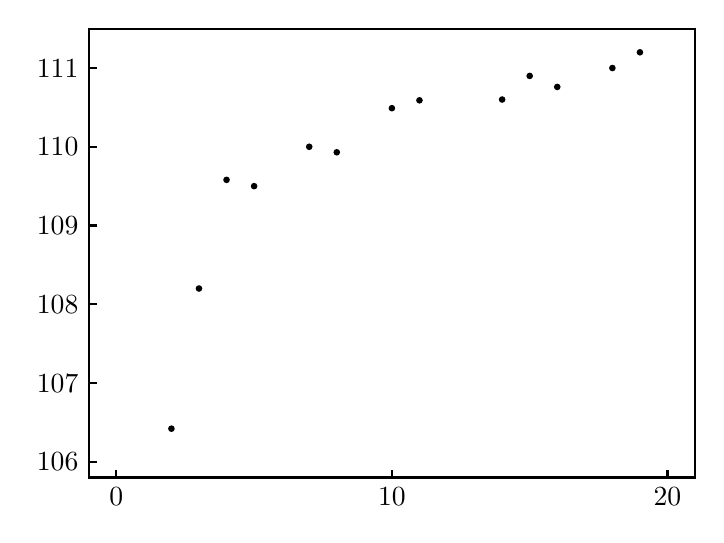
\begin{tikzpicture}[x=0.35cm,thick]
    \draw (-1,105.8) -- (21,105.8) -- (21,111.5)
       -- (-1,111.5) -- cycle;
    \foreach \x in {0,10,20}
      \draw (\x,105.8) node[below] {\x} -- ++ (0,0.1);
    \foreach \y in {106,...,111}
      \draw (-1,\y) node[left] {\y} -- ++ (0.3,0);
    \foreach \x/\y in {
      2/106.42, 3/108.20, 4/109.58, 5/109.50,
      7/110.00, 8/109.93, 10/110.49, 11/110.59,
      14/110.60, 15/110.90, 16/110.76, 18/111.00,
      19/111.20
    }
    \fill (\x,\y) circle (1.2pt);
  \end{tikzpicture}
    \caption{钢包质量与试验次数散点图}
    \label{fig:8.5.1}
    \end{figure}

    观测这 $13$ 个点构成的散点图,我们可以看到它们并不接近一条直线,用曲线拟合这些点应该是更恰当的.这里就涉及如何选择曲线函数形式的问题,首先,如果可由专业知识确定回归函数形式,则应尽可能利用专业知识.当若不能由专业知识加以确定函数形式,则可将散点图与一些常见的函数关系的图形进行比较,选择几个可能的函数形式,然后使用统计方法在这些函数形式之间进行比较,最后确定合适的曲线回归方程.为此,必须了解常见的曲线函数的图形,见图~\ref{fig:8.5.2}.

    \begin{figure}[!ht]
    \centering
    \begin{tabular}{c|c|c|c}
      \toprule
      函数名称 & 函数表达式 & 图像 & 线性化方法 \\
      \midrule
      \makecell{双曲线\\函\quad 数} & $\frac1y=a+\frac bx$
      &
      \begin{varwidth}{9cm}
        \begin{varwidth}[t]{4cm}
      \vspace{0pt}
       \begin{tikzpicture}[>=Stealth,scale=0.8]
    \draw [<->] (0,3) node[left] {$y$} -- (0,0) node [below left]{$O$} -- (3,0) node[below] {$x$};
    \draw [thick,domain=0.61:2.7] plot[samples=100](\x,{\x/(2*\x-1)});
    \draw [densely dashed] (0,0.5) node[left] {$\frac1a$}
      -- ++ (2.8,0)
      (0.5,0)node[below]{$-\frac ba$} -- ++ (0,2.87);
    \node[align=center] at (2.2,2.2) {$a>0$\\[1mm]$b>0$};
  \end{tikzpicture}
  \end{varwidth}%
  \begin{varwidth}[t]{4cm}
      \vspace{0pt}
  \begin{tikzpicture}[>=Stealth,scale=0.8]
    \draw [-Stealth] (0,-1) -- (0,2) node[left] {$y$};
    \draw [-Stealth] (-0.31,0)node[left]{$-\frac ba$} -- (0,0) node[below right] {$O$} -- (3,0) node[below] {$x$};
    \draw [domain = -0.2:2.7,thick] plot [samples=100] (\x,{3*\x/(2*\x+1)});
    \draw[densely dashed] (0,1.4)node[above right]{$\frac 1a$} -- ++ (2.8,0)
    (-0.31,-1) -- ++ (0,2.5);
  \end{tikzpicture}
  \end{varwidth}
      \end{varwidth}
      & \makecell{$v=\frac1y$\\$u=\frac1x$} \\
      \midrule
      幂函数 & $y=ax^b$ &
      \begin{varwidth}{4cm}
      \begin{tikzpicture}[>=Stealth,scale=0.8]
    \draw [<->] (0,3) node[left] {$y$} -- (0,0) node[below left] {$O$} -- (3,0) node[below] {$x$};
    \draw [thick,samples=100] plot [domain=0:1.3] (\x,{(\x)^3})
      plot [domain=0:1.3] ({(\x)^3},\x) (0,0) -- (1.8,1.8);
    \draw [densely dashed] (0,1) node[left] {$a$} -- (1,1) -- (1,0);
    \draw [->](0.7,2.5) node [above=0pt,inner sep=0pt]{$b>1$} -- (1.2,1.2^3);
    \draw [->](2.5,0.7)
    node [below=0pt,inner sep=0pt]{$0<b<1$} -- (1.2^3,1.2);
    \draw [->] (2.7,2.4)
    node [above=0pt,inner sep=0pt]{$b=1$} -- (1.8,1.8);
  \end{tikzpicture}
      \end{varwidth}
      \begin{varwidth}{4cm}
      \begin{tikzpicture}[>=Stealth,scale=0.8]
    \draw [<->] (0,3) node[left] {$y$} -- (0,0) node[below left] {$O$} -- (3,0) node[below] {$x$};
    \draw [thick,samples=100] plot [domain=0.4:2.5](\x,1/\x)
    plot [domain=0.63:2.4](\x,{1/(\x)^2}) plot [domain=0.63:2.4]
    ({1/(\x)^2},\x);
    \draw [densely dashed] (0,1) node[left] {$a$} -- (1,1)
      -- (1,0) node[below] {1};
    \draw [->] (1.2,2.8) node[above=0pt,inner sep=0pt]
      {$-1<b<0$} -- (1/2.4^2,2.4);
    \draw [->] (1.6,2.4) node[right=1pt,inner sep=0pt]
      {$b=-1$} -- (0.5,2);
    \draw [->] (2,2) node[right=1pt,inner sep=0pt]
      {$b<-1$} -- (0.8,1/0.8^2);
  \end{tikzpicture}
      \end{varwidth}
      & \makecell{$v=\ln y$\\$u=\ln x$} \\
      \midrule
      \multirow{2}*{\makecell{ 指\quad 数\\函\quad 数}} &
      $y=a\ee^{bx}$ &
      \begin{varwidth}{4cm}
      \begin{tikzpicture}[>=Stealth,scale=0.8]
    \draw [->] (-1.3,0) -- (0,0) node[below] {$O$} -- (1.7,0) node[below] {$x$};
    \draw [->] (0,0) -- (0,3) node[left] {$y$} ;
    \draw [domain=-0.9:1.4,samples=100,thick] plot (\x,{0.6*e^(\x)});
    \node at (-0.6,2) {$b>0$};
  \end{tikzpicture}
      \end{varwidth}
      \begin{varwidth}{4cm}
      \begin{tikzpicture}[>=Stealth,scale=0.8]
    \draw [->] (-1.7,0) -- (0,0) node[below] {$O$} -- (1.3,0) node[below] {$x$};
    \draw [->] (0,0) -- (0,3) node[left] {$y$} ;
    \draw [domain=-1.4:0.9,samples=100,thick] plot (\x,{0.6*e^(-\x)});
    \node at (0.6,2) {$b<0$};
  \end{tikzpicture}
      \end{varwidth}
      & \makecell{$v=\ln y$\\$u=x$} \\
      \cmidrule{2-4}
        & $y=a\ee^{b/x}$ &
        \begin{varwidth}{4cm}
      \begin{tikzpicture}[>=Stealth,scale=0.8]
    \draw [<->] (0,3) node[left] {$y$} -- (0,0) node[below left] {$O$} -- (3,0) node[below] {$x$};
    \draw[thick] (0,0) -- plot[domain=0.05:2.6,samples=100] (\x,{2.5*e^(-0.5/\x)});
    \draw [densely dashed] (0,2.1) node[left] {$a$} -- ++(2.5,0);
    \node at (2,2.5) {$b<0$};
  \end{tikzpicture}
      \end{varwidth}
      \begin{varwidth}{4cm}
      \begin{tikzpicture}[>=Stealth,scale=0.8]
    \draw [<->] (0,3) node[left] {$y$} -- (0,0) node[below left] {$O$} -- (3,0) node[below] {$x$};
    \draw[thick] plot[domain=0.2:2.2,samples=100] (\x,{5/(5*\x+0.9)});
    \draw [densely dashed] (0,0.35) node[left] {$a$}
     -- ++ (2.3,0);
    \node at (1.5,2.5) {$b>0$};
  \end{tikzpicture}
      \end{varwidth} & \makecell{$v=\ln y$\\$u=\frac1x$}\\
      \midrule
      \makecell{对\quad 数\\函\quad 数} & $y=a+b\ln x$ &
      \begin{varwidth}{9cm}
        \begin{varwidth}{4cm}
          \begin{tikzpicture}[>=Stealth,scale=0.8]
    \draw [->] (-0.3,0) -- (0,0) node[below left] {$O$}
      -- (2.7,0) node[below] {$x$};
    \draw [->] (0,-0.6) -- (0,2.4) node[left] {$y$};
    \draw [thick,domain=0.3:2.4,samples=100]
    plot (\x,{2-0.75/\x});
    \node at (1.5,2.2) {$b>0$};
  \end{tikzpicture}
        \end{varwidth}
        \begin{varwidth}{4cm}
        \begin{tikzpicture}[>=Stealth,scale=0.8]
    \draw [<->] (0,3) node[left] {$y$} -- (0,0) node[below left] {$O$} -- (3,0) node[below] {$x$};
    \draw [thick,samples=100,domain=0.4:2.5]
      plot(\x,-1+1/\x);
  \end{tikzpicture}
        \end{varwidth}
      \end{varwidth}
      & \makecell{$v=\ln y$\\$u=\frac1x$}\\
      \midrule
      \makecell{$S$\quad 形\\ 曲\quad 线} & $y=\frac1{a+b\ee^{-x}}$ &
      \begin{varwidth}{4cm}
       \begin{tikzpicture}[>=Stealth,scale=0.8]
    \draw [->] (-0.5,0) -- (0,0) node[below left] {$O$}
      -- (2.5,0) node[below] {$x$};
    \draw [->] (0,-0.3) -- (0,2.7) node[left] {$y$};
    \draw [thick,samples=100,domain=-0.25:2.4]
      plot(\x,{1/(0.5+3*e^(-3*\x))});
    \draw [densely dashed] (0,2.05) node[left] {$\frac1a$}
      -- ++ (2.4,0);
  \end{tikzpicture}
      \end{varwidth}
      & \makecell{$v=\frac1y$
      \\$u=\ee^{-x}$} \\
      \bottomrule
    \end{tabular}
    \caption{部分常见的曲线函数的图形}
    \label{fig:8.5.2}
    \end{figure}

    本例中,散点图呈现一个明显的向上且上凸的趋势,可能选择的函数关系有很多,比如,参照图~\ref{fig:8.5.2}, 我们可以给出如下四个曲线函数:
    \begin{align}
    1 &\quad 1 / y=a+b / x : \label{eq:8.5.1} \\
    2  &\quad  y=a+b \ln x ;  \label{eq:8.5.2}\\
    3  &\quad  y=a+b \sqrt{x} ; \label{eq:8.5.3} \\
    4  &\quad  y-100=a \cdot \ee^{-x / b}(b>0)\label{eq:8.5.4}
    \end{align}
    在初步选出可能的函数关系(即方程)后,我们必须解决两个问题:
    \begin{itemize}
        \item 如何估计所选方程中的参数?这在~\ref{ssec:8.5.2} 中讨论;
        \item 如何评价所选不同方程的优劣?这在~\ref{ssec:8.5.3} 中介绍.
    \end{itemize}
\end{example}

\subsection{参数估计}\label{ssec:8.5.2}

对形如~\eqref{eq:8.5.1} 式至~\eqref{eq:8.5.4} 式的非线性函数,参数估计最常用的方法是“线性化”方法,即通过某种变换,将方程化为一元线性方程的形式.

以~\eqref{eq:8.5.1} 式为例,为了能采用一元线性回归分析方法,我们作如下变换
\begin{equation*}
  u =1/x, \quad \nu =1/y,
\end{equation*}
则~\eqref{eq:8.5.1}的曲线函数就化为如下的直线
\begin{equation*}
  \nu = a + bu
\end{equation*}
这是理论回归函数. 对数据而言, 回归方程为
\begin{equation*}
\nu_i=a+b u_i+\varepsilon_i,
\end{equation*}
于是可用一元线性回归的方法估计出 $a,b$. 图~\ref{fig:8.5.3} 给出变换后的数据的散点图.

从图~\ref{fig:8.5.3} 上看出可以认为所有的点近似在一条直线上下被动,因此,建立一元线性回归方程是可行的.整个计算过程及估计列于表~\ref{tab:8.5.2} 和表~\ref{tab:8.5.3} 中.

\begin{figure}[htb]
    \centering
    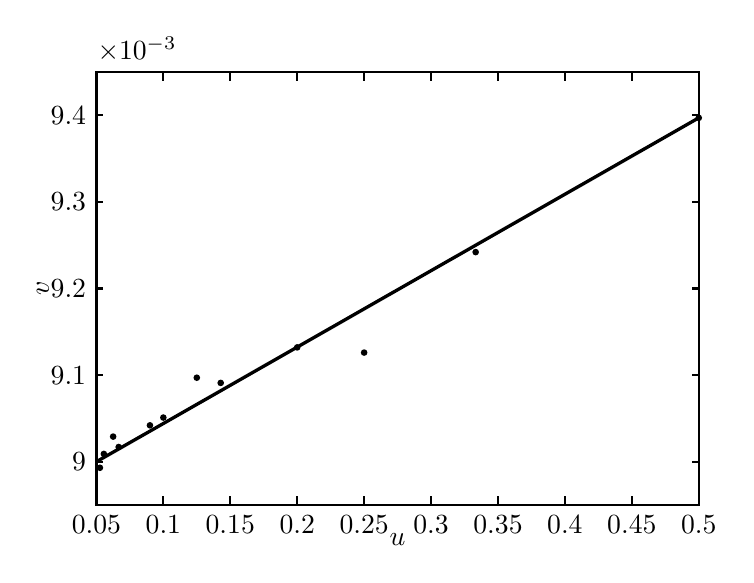
\begin{tikzpicture}[x=17cm,thick,y=11cm]
    \draw (0.05,8.95) -- (0.5,8.95) -- (0.5,9.45)
      -- (0.05,9.45) -- cycle;
    \foreach \x in {0.05,0.1,0.15,0.2,0.25,0.3,0.35,0.4,
    0.45,0.5}
      \draw (\x,8.95) node[below] {\x} -- ++ (0,0.01)
        (\x,9.45) -- ++ (0,-0.01);
    \foreach \y in {9,9.1,9.2,9.3,9.4}
      \draw (0.05,\y) node[left]{\y} -- ++ (0.005,0)
        (0.5,\y) -- ++ (-0.005,0);
    \draw (0.01,9.2) node[rotate=90] {$v$}
          (0.275,8.91) node {$u$}
          (0.05,9.45) node[anchor=south west,inner xsep=0pt] {$\times 10^{-3}$};
    \foreach \x/\y in {
      0.5/9.397, 0.333333/9.242, 0.25/9.126, 0.2/9.132,
      0.142857/9.091, 0.125/9.097, 0.1/9.051, 0.09/9.042,
      0.066667/9.017, 0.0625/9.029, 0.055556/9.009,
      0.052632/8.993
    }
    \fill (\x,\y) circle (1.2pt);
    \draw [very thick] (0.05,9) -- (0.5,9.397);
  \end{tikzpicture}
    \caption{变换后数据的散点图}
    \label{fig:8.5.3}
\end{figure}
% Table generated by Excel2LaTeX from sheet '1'
\begin{table}[!htbp]
  \renewcommand*{\arraystretch}{1.5}
    \centering
    \caption{钢包数据的变换值}
    \begin{tabularx}{0.8\linewidth}{ZZZZZZ}
        \toprule
     $x$      &  $y$      &  $u =1/x$  &  $\nu =1/y$  &  $\nu^2$  &  $u\nu$  \\\midrule
        2     & 106.42  & 0.500000  & 0.009397  & 0.250000  & 0.004698  \\
        3     & 108.20  & 0.333333  & 0.009242  & 0.111111  & 0.003081  \\
        4     & 109.58  & 0.250000  & 0.009126  & 0.062500  & 0.002281  \\
        5     & 109.50  & 0.200000  & 0.009132  & 0.040000  & 0.001826  \\
        7     & 110.00  & 0.142857  & 0.009091  & 0.020408  & 0.001299  \\
        8     & 109.93  & 0.125000  & 0.009097  & 0.015625  & 0.001137  \\
        10    & 110.49  & 0.100000  & 0.009051  & 0.010000  & 0.000905  \\
        11    & 110.59  & 0.090909  & 0.009042  & 0.008264  & 0.000822  \\
        14    & 110.60  & 0.071429  & 0.009042  & 0.005102  & 0.000646  \\
        15    & 110.90  & 0.066667  & 0.009017  & 0.004444  & 0.000601  \\
        16    & 110.76  & 0.062500  & 0.009029  & 0.003906  & 0.000564  \\
        18    & 111.00  & 0.055556  & 0.009009  & 0.003086  & 0.000501  \\
        19    & 111.20  & 0.052632  & 0.008993  & 0.002770  & 0.000473  \\
        \multicolumn{2}{c}{合计} & 2.050882  & 0.118267  & 0.537218  & 0.018835  \\
        \multicolumn{2}{c}{均值} & 0.15776 & 0.009097 &       &  \\\bottomrule
    \end{tabularx}%
    \label{tab:8.5.2}%
\end{table}%

% Table generated by Excel2LaTeX from sheet '1'
\begin{table}[!htb]
  \renewcommand*{\arraystretch}{1.5}
    \centering
    \caption{参数估计计算表}
    \begin{tabularx}{\linewidth}{ZZZ}
      \toprule
     $\sum u_i=2.050 88194$   &    $n=13$     &  $\sum \nu_i=0.11826672$  \\
     $\bar{u}=0.157 76015$   &       &  $ \bar{\nu} =0.009 097 44$  \\
     $\sum u_{i}^{2}=0.537 217 98$   &    $\sum u_i\nu_i=0.01883495$     &  \\
     $n\bar{u}=0.537 21798$   &   $n\overline{u\nu}=0.01865778$      &  \\
     $l_{\nu\nu}=0.21367054$   &   $l_{u\nu}=0.000 17717$      &  \\
        \multicolumn{3}{c}{ $\hat{b}=l_{u\nu }/l_{uu}=0.00082917$ } \\
        \multicolumn{3}{c}{ $\hat{a}\bar{\nu}-\bar{u}\hat{b}=0.00896663$ } \\
        \multicolumn{3}{c}{ $\displaystyle\therefore \hat{y}=\frac{x}{0.00082917+0.00896663.x}$ } \\[2ex]
        \bottomrule
    \end{tabularx}%
    \label{tab:8.5.3}%
\end{table}%
用类似的方法可以得出其他三个曲线回归方程, 它们分别是:
\begin{align*}
  & \hat{y}=106.3147+3.9466 \ln x, \\
  & \hat{y}=106.3013+1.1947 \sqrt{x}, \\
  & \hat{y}=100+11.7506 \mathrm{e}^{-1.1256 / x}.
\end{align*}

\subsection{曲线回归方程的比较}\label{ssec:8.5.3}

我们上面得到了四个曲线回归方程,在这四个方程中,哪一个更好一点呢?
通常可采用如下两个指标进行选择.
\begin{enumerate}
    \item 决定系数 $R^2$:类似于一元线性回归方程中相关系数,决定系数定义为:
    \begin{equation}
    R^{2}=1-\frac{\sum\left(y_{i}-\hat{y}_{i}\right)^{2}}{\sum\left(y_{i}-\bar{y}\right)^{2}}\label{eq:8.5.5}
    \end{equation} $R^2$ 越大,说明残差越小,回归曲线拟合越好, $R^2$ 从总体上给出一个拟合好坏程度的度量.
    \item 剩余标准差 $s$ :类似于一元线性回归中标准差的估计公式,此剩余标准差可用残差平方和来获得,即
    \begin{equation}
    s=\sqrt{\frac{\sum (y_i-\hat{y}_i)^2}{n-2}}\label{eq:8.5.6}
    \end{equation}
 $s$ 为诸观测点 $y_i$ 与由曲线给出的拟合值 $\hat{y}_i$ 间的平均偏离程度的度量, $s$ 越小,方程越好.
\end{enumerate}

在观测数据给定后,不同的曲线选择不会影响 $\sum_{i=1}^{n} (y_i-\bar{y}_i)^2$ 的取值,但会影响到残差平方和 $\sum_{i=1}^{n} (y_i-\hat{y}_i)^2$ 的取值.因此,对选择的曲线而言,决定系数和剩
余标准差都取决于残差平方和 $\sum_{i=1}^{n} (y_i-\hat{y}_i)^2$ ,从而,两种选择准则是一致的,只是从两个不同侧面作出评价.

表~\ref{tab:8.5.4} 给出第一个曲线回归方程的残差平方和的计算过程,由于 $n=13$ , $\sum_{i=1}^{13}(y_i-\bar{y})^2=0.5743$ ,故其决定系数及剩余标准差分别为:
\begin{equation*}
R^{2}=1-\frac{0.5743}{21.2105}=0.9729, \quad s=\sqrt{\frac{0.5743}{13-2}}=0.2285
\end{equation*}
% Table generated by Excel2LaTeX from sheet '1'
\begin{table}[htbp]
  \renewcommand*{\arraystretch}{1.5}
    \centering
    \caption{第一个方程的残整平方和计算表}
    \begin{tabular}{cccc|cccc}
        \toprule
     $y_i$   &  $\hat{y}_i$  &  $\hat{e}_i=y_{i} - \hat{y}_i$  &  $\hat{e}_i^2$  &  $y_i$   &  $\hat{y}_i$  &  $\hat{e}_i$  &  $\hat{e}_i^2$  \\\midrule
        106.42 & 106.596 & $-0.179$ & 0.030976 & 110.59 & 110.595 & $-0.00489$ & 0.000024 \\
        108.2 & 108.19 & 0.010252 & 0.000105 & 110.6 & 110.793 & $-0.193$ & 0.037249 \\
        109.52 & 109.005 & 0.575373 & 0.331054 & 110.9 & 110.841 & 0.059 & 0.003481 \\
        109.5 & 109.499 & 0.00526 & 0.000000 & 110.76 & 110.884 & $-0.124$ & 0.015376 \\
        110   & 110.071 & $-0.07054$ & 0.004976 & 111   & 110.955 & 0.045 & 0.002025 \\
        109.93 & 110.25 & $-0.32023$ & 0.102544 & 111.2 & 110.984 & 0.216 & 0.046656 \\
        110.49 & 110.503 & $-0.01277$ & 0.000163 & \multicolumn{3}{c}{和} & 0.5743 \\\bottomrule
    \end{tabular}%
    \label{tab:8.5.4}%
\end{table}%
其他三个方程的决定系数及剩余标准差可同样计算, 我们将它们列在表~\ref{tab:8.5.5} 中.
\begin{table}[!htb]
    \centering
    \caption{四种曲线回归的决定系数及剩余标准差}
    \begin{tabular}{ccccc}
    \toprule
    模型编号  & 1      & 2      & 3      & 4      \\
    \midrule
    $R^2$    & 0.9729 & 0.8773 & 0.7551 & 0.9623 \\
    $s$      & 0.2285 & 0.4864 & 0.6437 & 0.2696 \\
    \bottomrule
    \end{tabular}%
    \label{tab:8.5.5}%
\end{table}%

从表~\ref{tab:8.5.5} 中可以看出,第一个曲线方程的决定系数最大,剩余标准差最小,在这四个曲线回归方程中,不论用哪个标准,都是第一个方程拟合得最好.因此,近似得比较好的定量关系式就是
\begin{equation*}
\hat{y}=\frac{x}{0.00082917 + 0.008 96663 x}
\end{equation*}

\vskip4ex

\begin{xiti}
    \item 设曲线函数形式为 $y = a + b \ln x$, 试给出一个变换将之化为一元线性回归的形式.
    \item 设曲线函数形式为 $y = a + b \sqrt{x}$, 试给出一个变换将之化为一元线性回归的形式.
    \item 设曲线函数形式为 $y - 100 = a \ee^{-x/b} (b > 0)$, 试给出一个变换将之化为一元线性回归的形式.
    \item 设曲线函数形式为 $y = a + \ee^{bz}$, 问能否找到一个变换将之化为一元线性回归的形式,若能,试给出;若不能,说明理由.
    \item 设曲线函数形式为 $\displaystyle y = \frac{1}{a + b\ee^{-x}}$, 问能否找到一个变换将之化为一元线性回归的形式,若能,试给出;若不能,说明理由.
    \item 设曲线函数形式为 $y = a \ee^{b/x}$ ,问能否找到一个变换将之化为一元线性回归的形式,若能,试给出;若不能,说明理由.
    \item 为了检验 $X$ 射线的杀菌作用,用 \SI{200}{\kV} 的 $X$ 射线照射杀菌,每次照射 \SI{6}{\minute}, 照射次数为 $x$ ,照射后所剩细菌数为 $y$ ,下表是一组试验结果

    \begin{center}
    \begin{tabularx}{0.8\linewidth}{YY|YY|YY}
  \toprule
    x     & y     & x     & y     & x     & y \\
  \midrule
    1     & 783   & 8     & 154   & 15    & 28 \\
    2     & 621   & 9     & 129   & 16    & 20 \\
    3     & 433   & 10    & 103   & 17    & 16 \\
    4     & 431   & 11    & 72    & 18    & 12 \\
    5     & 287   & 12    & 50    & 19    & 9  \\
    6     & 251   & 13    & 43    & 20    & 7  \\
    7     & 175   & 14    & 31    &       &    \\
  \bottomrule
    \end{tabularx}
    \end{center}
    根据经验知道 $y$ 关于 $x$ 的曲线回归方程形如
    \begin{equation*}
      y=a\ee^{bx},
    \end{equation*}
    试给出具体的回归方程,并求其对应的决定系数 $R^2$ 和剩余标准差 $s$.
\end{xiti} 